\chapter{Foundations: Cultural Internalisation - Towards Vygotskian Autotelic Agents}
\label{chap:foundation_vaai}
\minitoc

\section{Developmental Machine Learning and Intrinsic motivations}

% Human learning is great, we’d like to train agents to show similar learning abilities and behavior
Building autonomous machines that can explore large environments, discover interesting interactions and learn open-ended repertoires of skills is a long-standing goal in artificial intelligence. Humans are remarkable examples of this lifelong, open-ended learning. They learn to recognize objects and crawl as infants, then learn to ask questions and interact with peers as children. Across their lives, humans build a large repertoire of diverse skills from a virtually infinite set of possibilities. What is most striking, perhaps, is their ability to invent and pursue their own problems, using internal feedback to assess completion. We would like to build artificial agents able to demonstrate equivalent lifelong learning abilities.

% We can think of two fields targeting the problem of learning behaviors

We can think of two approaches to this problem: developmental approaches, in particular developmental robotics, and reinforcement learning (\rl). Developmental robotics takes inspirations from artificial intelligence, developmental psychology and neuroscience to model cognitive processes in natural and artificial systems \cite{asada2009cognitive,cangelosi2015developmental}. Following the idea that intelligence should be \textit{embodied}, robots are often used to test learning models. Reinforcement learning, on the other hand, is the field interested in problems where agents learn to behave by experiencing the consequences of their actions under the form of rewards and costs. As a result, these agents are not explicitly taught, they need to learn to maximize cumulative rewards over time by trial-and-error \cite{sutton2018reinforcement}. While developmental robotics is a field oriented towards answering particular questions around sensorimotor, cognitive and social development (\eg how can we model language acquisition?), reinforcement learning is a field organized around a particular technical framework and set of methods.

% RL - Standard, multi-goal, limits, awesome achievements

Now powered by deep learning optimization methods leveraging the computational efficiency of large computational clusters, \rl algorithms have recently achieved remarkable results including, but not limited to, learning to solve video games at a super-human level \cite{mnih2015human}, to beat chess and go world players \cite{silver2016mastering}, or even to control stratospheric balloons in the real world \cite{bellemare2020autonomous}.

Although standard \rl problems often involve a single agent learning to solve a unique task, \rl researchers  extended \rl problems to \textit{multi-goal \rl problems}. Instead of pursuing a single goal, agents can now be trained to pursue goal distributions \cite{kaelbling1993learning,sutton2011horde,schaul2015universal}. As the field progresses, new goal representations emerge: from the specific goal states to the high-dimensional goal images or the abstract language-based goals \cite{Luketina2019}. However, most approaches still fall short of modeling the learning abilities of natural agents because they train them to solve predefined sets of tasks, via external and hand-defined learning signals.

% Dev robotics - good approach, formulate the right problem, but not awesome achievements
Developmental robotics directly aims to model children learning and, thus, takes inspiration from the mechanisms underlying autonomous behaviors in humans. Most of the time, humans are not motivated by external rewards but spontaneously explore their environment to discover and learn about what is around them. This behavior seems to be driven by \textit{intrinsic motivations} (\ims) a set of brain processes that motivate humans to explore for the mere purpose of experiencing novelty, surprise or learning progress \cite{berlyne1966curiosity,gopnik1999scientist,kidd2015psychology,oudeyer2016evolution,gottlieb2018towards}.

The integration of \ims into artificial agents thus seems to be a key step towards autonomous learning agents \cite{schmidhuber1991possibility,kaplan2007search}. In developmental robotics, this approach enabled sample efficient learning of high-dimensional motor skills in complex robotic systems \cite{santucci2020intrinsically}, including locomotion \cite{baranes2013active,martius2013information}, soft object manipulation \cite{rolf2013efficient,nguyen2014socially}, visual skills \cite{lonini2013robust} and nested tool use in real-world robots \cite{imgep}. Most of these approaches rely on \textit{population-based} optimization algorithms, non-parametric models trained on datasets of (policy, outcome) pairs. Population-based algorithms cannot leverage automatic differentiation on large computational clusters, often demonstrate limited generalization capabilities and cannot easily handle high-dimension perceptual spaces (\eg images) without hand-defined input pre-processing. For these reasons, developmental robotics could benefit from new advances in deep \rl.

% Recently, we’ve been observing a convergence between the two with ideas from dev rob being integrated within RL
%     frameworks, and RL tools being used for dev rob objectives.
Recently, we have been observing a convergence of these two fields, forming a new domain that we propose to call \textit{developmental reinforcement learning}, or more broadly \textit{developmental artificial intelligence}. Indeed, \rl researchers now incorporate fundamental ideas from the developmental robotics literature in their own algorithms, and reversely developmental robotics learning architecture are beginning to benefit from the generalization capabilities of deep \rl techniques. These convergences can mostly be categorized in two ways depending on the type of intrinsic motivation (\ims) being used \cite{oudeyer2007intrinsic}:
\begin{itemize}
    \item
    \textbf{Knowledge-based IMs} are about prediction. They compare the situations experienced by the agent to its current knowledge and expectations, and reward it for experiencing dissonance (or resonance). This family includes \ims rewarding prediction errors \cite{schmidhuber1991possibility,pathak2017curiosity}, novelty \cite{bellemare2016unifying,burda2018exploration,raileanu2020ride}, surprise \cite{achiam2017surprise}, negative surprise \cite{berseth2019smirl}, learning progress \cite{lopes2012exploration,kim2020active} or information gains \cite{houthooft2016vime}, see a review in \cite{linke2019adapting}. This type of \im is often used as an auxiliary reward to organize the exploration of agents in environments characterized by sparse rewards. It can also be used to facilitate the construction of world models \cite{lopes2012exploration,kim2020active,sekar2020planning}.
    \item
    \textbf{Competence-based IMs}, on the other hand, are about control. They reward agents to solve self-generated problems, to achieve self-generated goals. In this category, agents need to represent, select and master self-generated goals. As a result, competence-based \ims were often used to organize the acquisition of repertoires of skills in task-agnostic environments \cite{baranes2010intrinsically,baranes2013active,santucci2016grail,forestier2016modular,nair2018visual,warde2018unsupervised,curious,blaes2019control,pong2019skew,imagine}. Just like knowledge-based \ims, competence-based \ims organize the exploration of the world and, thus, might be used to train world models \cite{baranes2013active,chitnis2020glib} or facilitate learning in sparse reward settings \cite{geppg}. We propose to use the adjective \textbf{autotelic}, from the Greek \textit{auto} (self) and \textit{telos} (end, goal), to characterize agents that are intrinsically motivated to represent, generate, pursue and master their own goals (\ie that are both intrinsically motivated and goal-conditioned).
\end{itemize}

\rl algorithms using \textit{knowledge-based} \ims leverage ideas from developmental robotics to solve standard \rl problems. On the other hand, \rl algorithms using competence-based \ims organize exploration around self-generated goals and can be seen as targeting a developmental robotics problem: the \textit{open-ended and self-supervised acquisition of repertoires of diverse skills}. 
 
\textit{Intrinsically Motivated Goal Exploration Processes} (\imgep) is the family of autotelic algorithms that bake competence-based \ims into learning agents \cite{imgep}. \imgep agents generate and pursue their own goals as a way to explore their environment, discover possible interactions and build repertoires of skills. This framework emerged from the field of developmental robotics \cite{oudeyer2007intrinsic,baranes2009proximo,baranes2010intrinsically,rolf2010goal} and originally leveraged population-based learning algorithms (\popimgep) \cite{baranes2009r,baranes2013active,forestier2016modular,imgep}. 

Recently, goal-conditioned \rl agents were also endowed with the ability to generate and pursue their own goals and learn to achieve them via self-generated rewards. We call this new set of autotelic methods \rlimgeps. In contrast, one can refer to externally-motivated goal-conditioned \rl agents as \rlemgeps.


\begin{figure}[h]
    \centering
    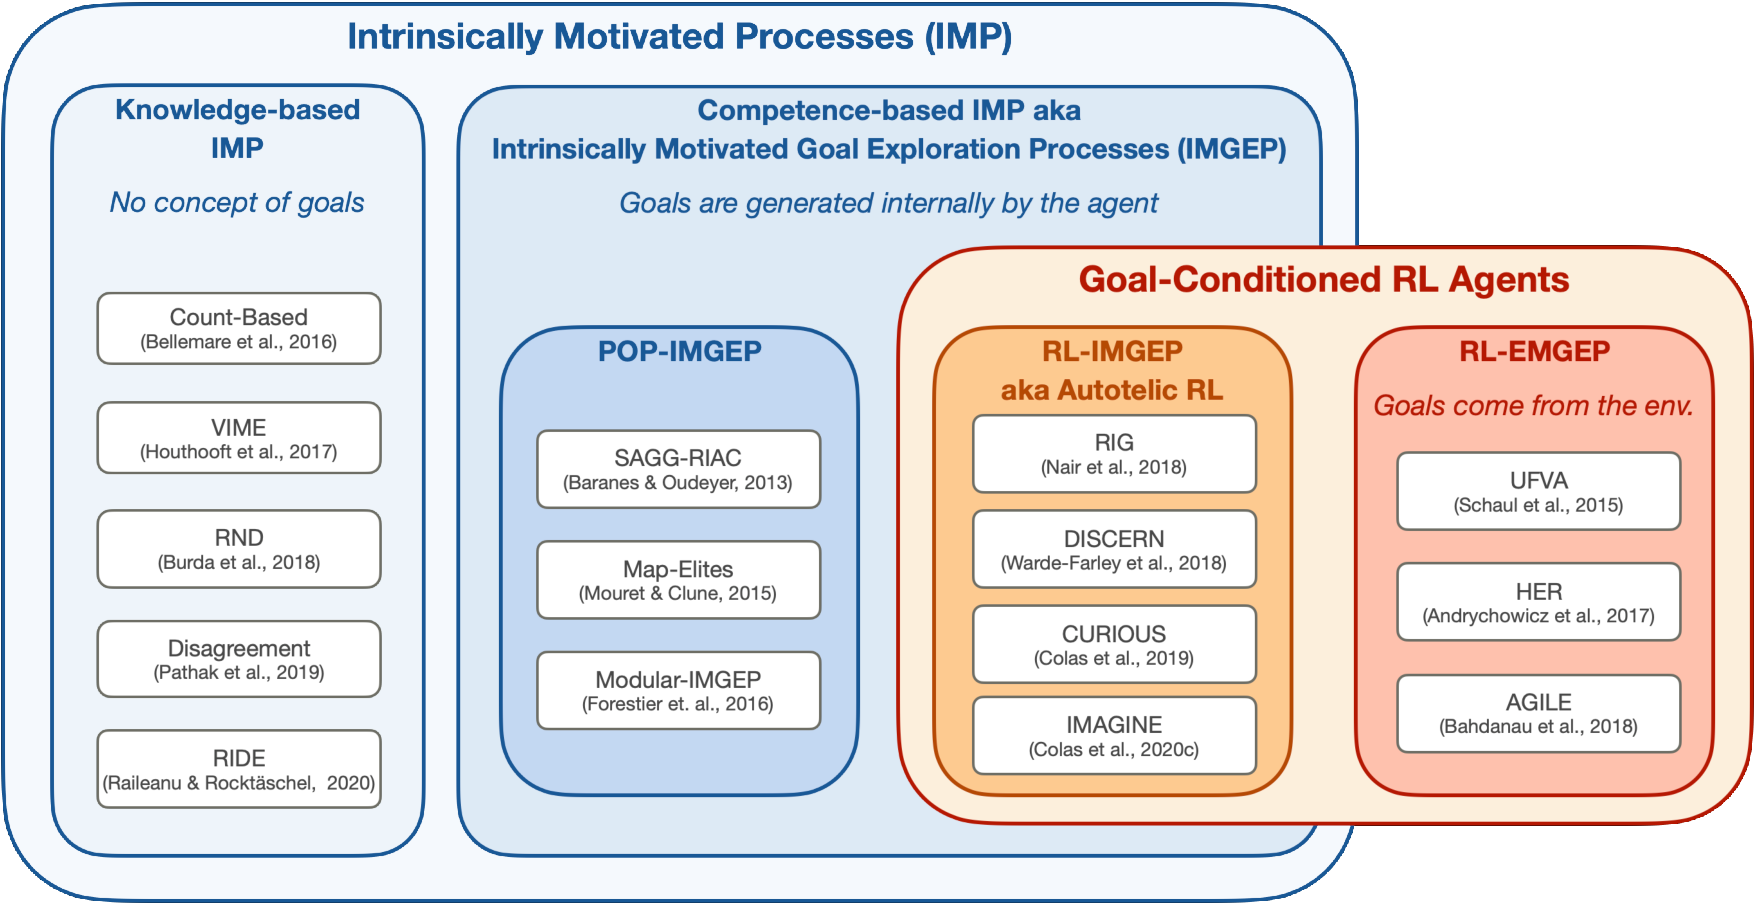
\includegraphics[width=\textwidth]{survey/scope5.pdf}
    \caption{A typology of intrinsically-motivated and/or goal-conditioned \rl approaches. \popimgep, \rlimgep
    and \rlemgep refer to \textit{population-based intrinsically motivated goal exploration processes}, 
        \textit{\textsl{\rl}-based} \textsl{\imgep} and \textit{\textsl{\rl}-based externally motivated goal exploration
        processes} respectively. \popimgep, \rlimgep and \rlemgep all represent goals, but knowledge-based \ims
        do not. While \imgeps (\popimgep and \rlimgep) generate their own goals, \rlemgeps require
        externally-defined goals. This paper is interested in \rlimgeps, autotelic methods at the intersection of
        \textit{goal-conditioned \rl agents} and \textit{intrinsically motivated processes} that train learning
        agents to generate and pursue their own goals with goal-conditioned \rl algorithms. }
    \label{fig:scope}
\end{figure}


\section{From Reinforcement to Autotelic Learning}
\todo{select some concepts to include in the introduction}
\todo{clean section and sub}


% This is what this survey is about
This paper proposes a formalization and a review of the \rlimgep algorithms at the convergence of \rl methods and developmental robotics objectives. Figure~\ref{fig:scope} proposes a visual representation of intrinsic motivations approaches (knowledge-based \ims vs competence-based \ims or \imgeps) and goal-conditioned \rl (externally vs intrinsically motivated). Their intersection is the family of autotelic algorithms that train agents to generate and pursue their own goals by training goal-conditioned policies. 

We define goals as the combination of a compact goal representation and a goal-achievement function to measure progress. This definition highlights new challenges for autonomous learning agents. While traditional \rl agents only need to learn to achieve goals, \rlimgep agents also need to learn to represent them, to generate them and to measure their own
progress. After learning, the resulting goal-conditioned policy and its associated goal space form a \textit{repertoire of skills}, a repertoire of behaviors that the agent can represent and control. We believe organizing past goal-conditioned \rl algorithms at the convergence of developmental robotics and \rl into a common classification and towards the resolution of a common problem will help organize future research.


\begin{tcolorbox}
\small
\paragraph{Definitions}
\begin{itemize}
    \item \textit{\textbf{Goal}}: ``a cognitive representation of a future object that the organism is committed to approach \cite{elliot2008goal}.'' In \rl, this takes the form of a (embedding, goal-achievement function) pair, see Section~\ref{sec:goals}.
    \item \textit{\textbf{Skill}}: the association of a goal and a policy to reach it, see Section~\ref{sec:im_pb}.
    \item \textit{\textbf{Goal-achievement function}}: a function that measures progress towards a goal (also called goal-conditioned reward function), see Section~\ref{sec:goals}.
    \item \textit{\textbf{Goal-conditioned policy}}: a function that generates the next action given the current state and the goal, see Section~\ref{sec:im_pb_solution}.
    \item \textit{\textbf{Autotelic}}: from the Greek \textit{auto} (self) and \textit{telos} (end, goal), characterizes agents that generate their own goals and learning signals. In is equivalent to \textit{intrinsically motivated and goal-conditioned}.
\end{itemize}
\end{tcolorbox}


%\textbf{Scope of the survey.}
%We are interested in algorithms from the \rlimgep family as algorithmic tools to enable agents to acquire repertoires of skills in an open-ended and self-supervised setting. Externally motivated goal-conditioned \rl approaches do not enable agents to generate their own goals and thus cannot be considered autotelic (\imgeps). However, these approaches can often be converted into autotelic \rlimgeps by integrating the goal generation process within the agent. For this reason, we include some \rlemgeps approaches when they present interesting mechanisms that can directly be leveraged in autotelic agents. 
%
%%what’s not covered and why
%\textbf{What is not covered.} This survey does not discuss some related but distinct approaches such as multi-task \rl \cite{caruana1997multitask}, \rl with auxiliary tasks \cite{riedmiller2018learning,jaderberg2016reinforcement} and \rl with knowledge-based \ims \cite{bellemare2016unifying,pathak2017curiosity,burda2018exploration}. None of these approaches do represent goals or see the agent's behavior affected by goals. The subject of intrinsically motivated goal-conditioned \rl also relates to \textit{transfer learning} and \textit{curriculum learning}. This survey does not cover transfer learning approaches, but interested readers can refer to \cite{taylor2009transfer}. It  discusses automatic curriculum learning approaches that organize the generation of goals according to the agent's abilities in Section~\ref{sec:survey_generation} but, for a broader picture on the topic, readers can refer to the recent review \cite{portelas2020automatic}. Finally, this survey does not review policy learning methods but only focuses on goal-related mechanisms. Indeed, the choice of mechanisms to learn to represent and select goals is somewhat orthogonal to the algorithms used to learn to achieve them. Since the policy learning algorithms used in \rlimgep architectures do not differ significantly from standard \rl and goal-conditioned \rl approaches, this survey focuses on goal-related mechanisms, specific to \rlimgeps.
%
%\textbf{Survey organization.} We start by presenting some background on the formalization of \rl and multi-goal \rl problems and the corresponding algorithms to solve them (Section~\ref{sec:background}). We then build on these foundations to formalize the \textit{intrinsially motivated skills acquisition problem} and propose a computational framework to tackle it: \textit{\textsl{\rl}-based intrinsically motivated goal exploration processes} (Section~\ref{sec:im_pb_solution}). Once this is done, we organize the surveyed literature along three axes: 1) What are the different types of goal representations? (Section~\ref{sec:survey_goal_rep}); 2) How can we learn goal representations? (Section~\ref{sec:survey_learning_goal_rep}) and 3) How can we prioritize goal selection? (Section~\ref{sec:survey_generation}). We finally close the survey on a discussion of open challenges for developmental reinforcement learning (Section~\ref{sec:future}).

%\os{On pourrait peut-être mentionner qu'on ne couvre pas le cas (rarement étudié) où chaque tâche utilise sa propre
%    state action representation (cf. \cite{doncieux2018open}).}

% % % % % % % % % % % % % % % % % % % % % % % % % % %
% The Intrinsically Motivated Goal Exploration Problem
% % % % % % % % % % % % % % % % % % % % % % % % % % % 


\subsection{The Intrinsically Motivated Skills Acquisition Problem and the RL-IMGEP Framework}
\label{sec:im_pb_solution}
This section builds on the multi-goal \rl problem to formalize the \textit{intrinsically motivated skills acquisition problem}, in which goals are not externally provided to the agents but must be represented and generated by them (Section~\ref{sec:im_pb}). The following section discusses how to evaluate competency in such an open problem (Section~\ref{sec:eval}). Finally, we then propose an extension of the goal-conditioned \rl framework to tackle this problem: \textit{\textsl{rl}-based intrinsically motivated goal exploration process} framework (\rlimgep, Section~\ref{sec:gcimgep_solutions}). 

\paragraph{The Intrinsically Motivated Skills Acquisition Problem}
\label{sec:im_pb}
In the \textit{intrinsically motivated skills acquisition problem}, the agent is set in an open-ended environment without any pre-defined goal and needs to acquire a repertoire of skills. Here, a skill is defined as the association of a goal embedding $z_g$ and the policy to reach it $\Pi_g$. A repertoire of skills is thus defined as the association of a repertoire of goals $\m{G}$ with a goal-conditioned policy trained to reach them $\Pi_\m{G}$. The intrinsically motivated skills acquisition problem can now be modeled by a reward-free \mdp $\m{M}\,=\,\{\m{S},\, \m{A},\, \m{T},\, \rho_0\}$ that only characterizes the agent, its environment and their possible interactions. Just like children, agents must be autotelic, \ie they should learn to represent, generate, pursue and master their own goals.


\label{sec:eval}
\paragraph{Evaluating RL-IMGEP Agents. } 

Evaluating agents is often trivial in reinforcement learning. Agents are trained to maximize one or several pre-coded reward functions\,---\,the set of possible interactions is known in advance. One can measure generalization abilities by computing the agent's success rate on a held-out set of testing goals. One can measure exploration abilities via several metrics such as the count of task-specific state visitations.

In contrast, autotelic agents evolve in open-ended environments and learn to represent and form their own set of skills. In this context, the space of possible behaviors might quickly become intractable for the experimenter, which is perhaps the most interesting feature of such agents. For these reasons, designing evaluation protocols is not trivial.

The evaluation of such systems raises similar difficulties as the evaluation of task-agnostic content generation systems like Generative Adversarial Networks (\gan) \cite{goodfellow2014generative} or self-supervised language models \cite{devlin2019bert,brown2020language}. In both cases, learning is \textit{task-agnostic} and it is often hard to compare models in terms of their outputs (\eg comparing the quality of \gan output images, or comparing output repertoires of skills in autotelic agents).

One can also draw parallel with the debate on the evaluation of open-ended systems in the field of \textit{open-ended evolution} \cite{hintze_open-endedness_2019,stanley_role_2016,stanley_why_2019}. In both cases, a \textit{good} system is expected to generate more and more original solutions such that its output cannot be predicted in advance. But what does \textit{original} mean, precisely? \cite{stanley_role_2016} argues that subjectivity has a role to play in the evaluation of open-ended systems. Indeed, the notion of \textit{interestingness} is tightly coupled with that of \textit{open-endedness}. What we expect from our open-ended systems, and of our \rlimgep agents in particular, is to generate more and more behaviors that \textit{we} deem interesting. This is probably why the evaluation of content generators often include human studies. Our end objective is to generate interesting artefacts for us; we thus need to evaluate open-ended processes ourselves, subjectively.

Our end goal would be to interact with trained \rlimgep directly, to set themselves goals and test their abilities. The evaluation would need to adapt to the agent's capabilities. As Einstein said \textit{``If you judge a fish by its ability to climb a tree, it will live its whole life believing that it is stupid.''}. \rlimgep need to be evaluated by humans looking for their area of expertise, assessing the width and depth of their capacities in the world they were trained in. This said, science also requires more objective evaluation metrics to facilitate the comparison of existing methods and enable progress. Let us list some evaluation methods measuring the competency of agents via proxies:

\begin{itemize}
    \item \textbf{Measuring exploration:} one can compute task-agnostic exploration proxies such as the entropy of the
    visited state distribution, or measures of state coverage (\eg coverage of the high-level x-y state space in mazes) \cite{goalgan}. Exploration can also be measured as the number of interactions from a set of \textit{interesting} interactions defined subjectively by the experimenter \cite<\eg interactions with objects in>{imagine}.
    \item \textbf{Measuring generalization:} The experimenter can subjectively define a set of relevant target goals
    and prevent the agent from training on them. Evaluating agents on this held-out set at test time provides a measure of generalization \cite{ruis2020benchmark}, although it is biased towards what the experimenter assesses as \textit{relevant} goals.
    \item \textbf{Measuring transfer learning:} The intrinsically motivated exploration of the environment can be seen as a pre-training phase to bootstrap learning in a subsequent downstream task. In the downstream task, the agent is trained to achieve externally-defined goals. We report its performance and learning speed on these goals. This is akin to the evaluation of self-supervised language models, where the reported metrics evaluate performance in various downstream tasks \cite{brown2020language}. In this evaluation setup, autotelic agents can be compared to task-specific agents. Ideally, autotelic agents should benefit from their open-ended learning process to outperform task-specific agents on their own tasks. This said, performance on downstream tasks remains an evaluation proxy and should not be seen as the explicit \textit{objective} of the skill discovery phase. Indeed, in humans, skill discovery processes do not target any specific future task, but emerged from a natural evolutionary process maximizing reproductive success, see a discussion in \cite{singh2010intrinsically}.
    \item
    \textbf{Opening the black-box:} Investigating internal representations learned during intrinsically motivated exploration is often informative. One can investigate properties of the goal generation system (\eg does it generate out-of-distribution goals?), investigate properties of the goal embeddings (\eg are they disentangled?). One can also look at the learning trajectories of the agents across learning, especially when they implement their own curriculum learning \cite{goalgan,curious,blaes2019control,pong2019skew,akakzia2020decstr}.
    \item
    \textbf{Measuring robustness:} Autonomous learning agents evolving in open-ended environment should be robust to a variety of properties than can be found in the real-world. This includes very large environments, where possible interactions might vary in terms of difficulty (trivial interactions, impossible interactions, interactions whose result is stochastic thus prevent any learning progress). Environments can also include distractors (\eg non-controllable objects) and various forms of non-stationarity. Evaluating learning algorithms in various environments presenting each of these properties allows to assess their ability to solve the corresponding challenges.
\end{itemize}

 
%\newpage
\subsection{RL-Based Intrinsically Motivated Goal Exploration Processes}
\label{sec:gcimgep_solutions}
Until recently, the \imgep family was powered by population-based algorithms (\popimgep). The emergence of goal-conditioned \rl approaches that generate their own goals gave birth to a new type of \imgeps: the \rl-based \imgeps (\rlimgep). This section builds on traditional \rl and goal-conditioned \rl algorithms to give a general definition of intrinsically motivated goal-conditioned \rl algorithms (\rlimgep).

\rlimgep are intrinsically motivated versions of goal-conditioned \rl algorithms. They need to be equipped with mechanisms to represent and generate their own goals in order to solve the intrinsically motivated skills acquisition problem, see Figure~\ref{fig:goal_directed_rl}. Concretely, this means that, in addition to the goal-conditioned policy, they need to learn: 1)~to represent goals $g$ by compact embeddings $z_g$; 2)~to represent the support of the goal distribution, also called \textit{goal space} $\m{Z}_\m{G}=\{z_g\}_{g\in\m{G}}$; 3)~a goal distribution from which targeted goals are sampled $\m{D}(z_g)$; 4)~a goal-conditioned reward function $\m{R}_\m{G}$. In practice, only a few architectures tackle the four learning problems above. 

In this survey, \textbf{we call \textit{autotelic} any architecture where the agent selects its own goals (learning problem 3)}. Simple autotelic agents assume pre-defined goal representations (1), the support of the goals distribution (2) and goal-conditioned reward functions (4). As autotelic architectures tackle more of the 4 learning problems, they become more and more advanced. As we will see in the following sections, many existing works in goal-conditioned \rl can be formalized as autotelic agents by including goal sampling mechanisms \textit{within the definition of the agent}. 

With a developmental perspective, one can reinterpret existing work through the autotelic \rl framework. Let us take an example. The \textsc{agent$_{57}$} algorithm automatically selects a parameter to balance the intrinsic and extrinsic rewards of the agent at the beginning of each training episode \cite{badia2020agent57}. The authors do not mention the concept of \textit{goal} but instead present this mechanism as a form of reward shaping technique independent from the agent. With a developmental perspective, one can interpret the mixing parameter as a goal embedding. Replacing the sampling mechanism within the boundaries of the agent, \textsc{agent$_{57}$} becomes autotelic. It is intrinsically motivated to sample and target its own goals; \ie to define its own reward functions (here mixtures of intrinsic and extrinsic reward functions). 

Algorithm~\ref{algo:IMGEP} details the pseudo-code of \rlimgep algorithms. Starting from randomly initialized modules and memory, \rlimgep agents enter a standard \rl interaction loop. They first observe the context (initial state), then sample a goal from their goal sampling policy. Then starts the proper interaction. Conditioned on their current goal embedding, they act in the world so as to reach their goal, \ie to maximize the cumulative rewards generated by the goal-conditioned reward function. After the interaction, the agent can update all its internal models. It learns to represent goals by updating its goal embedding function and goal-conditioned reward function, and improves its behavior towards them by updating its goal-conditioned policy. 

\begin{figure}[h]
    \centering
    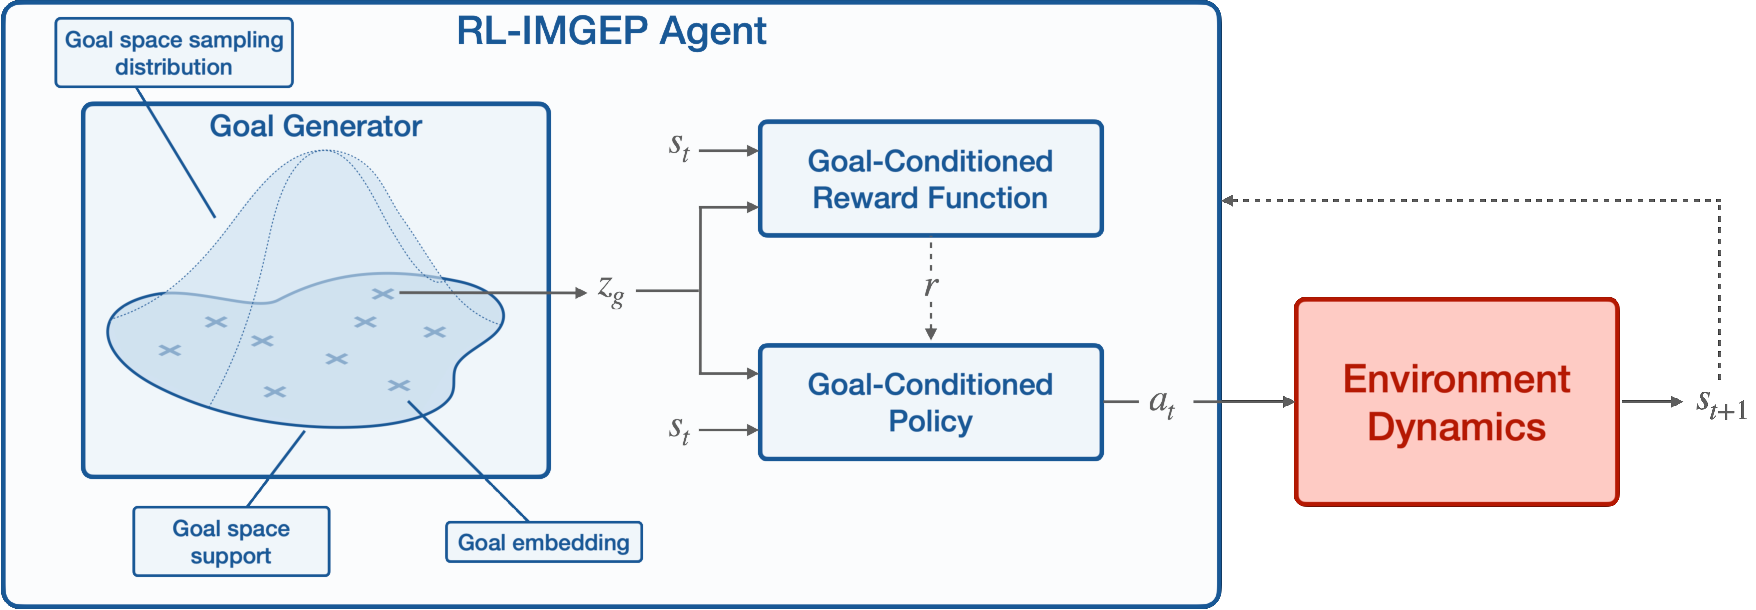
\includegraphics[width=0.95\textwidth]{survey/goal.pdf}
    \caption{Representation of the different learning modules in a \rlimgep algorithm. In contrast, externally     motivated goal exploration processes (\rlemgeps) only train the goal-conditioned policy and assume     \textit{external} goal generator and goal-conditioned reward function. Learning goal embeddings, goal space
    support and goal-conditioned reward functions are all about learning to \textit{represent goals}. Learning a
    sampling distribution is about learning to \textit{prioritize their selection}.}
    \label{fig:goal_directed_rl}
\end{figure}

This surveys focuses on the mechanisms specific to \rlimgep agents, \ie mechanisms that handle the representation, generation and selection of goals. These mechanisms are mostly orthogonal to the question of how to reach the goals themselves, which often relies on existing goal-conditioned algorithms, but can also be powered by imitation learning, evolutionary algorithms or other control and planning methods. Section~\ref{sec:survey_goal_rep} first presents a typology of goal representations used in the literature, before Sections~\ref{sec:survey_learning_goal_rep}~and~\ref{sec:survey_generation} cover existing methods to learn to represent and prioritize goals respectively. 



\noindent\begin{minipage}{\textwidth}
   \centering
   \begin{minipage}{.6\textwidth}
        \begin{algorithm}[H]
            \small
        	\caption{~ Autotelic Agent with RL-IMGEP}
        	\label{algo:IMGEP}
        	\begin{algorithmic}[1]
            	\REQUIRE environment $\m{E}$
            	\STATE \textbf{Initialize} empty memory $\m{M}$,goal-conditioned policy $\Pi_\m{G}$, goal-conditioned reward $R_\m{G}$,goal space $\m{Z}_\m{G}$, goal sampling policy $GS$.
            	
            	\LOOP
            	
%                \LineCommentConttwo{\textit{Observe context}}
                \STATE Get initial state: $s_0 \leftarrow \m{E}$.reset()
%            	\LineCommentCont{\textit{Sample goal}}
            	\STATE Sample goal embedding $z_g=GS(s_0, \m{Z}_\m{G})$.
%            	\LineCommentCont{\textit{Roll-out goal-conditioned policy}}
            	\STATE Execute a roll-out with $\Pi_g=\Pi_\m{G}(\cdot \mid z_g)$
            	\STATE Store collected transitions $\tau=(s,a,s')$ in $\m{M}$.
%            	\LineCommentCont{\textit{Update internal models}}
                \STATE Sample a batch of $B$ transitions: $\m{M}\sim \{(s,a,s')\}_B$.
                \STATE Perform Hindsight Relabelling $\{(s,a,s',z_g)\}_B$.
                \STATE Compute internal rewards $r=R_\m{G}(s,a,s'\mid z_g)$.
            	\STATE Update policy $\Pi_\m{G}$ via \rl on $\{(s,a,s',z_g,r)\}_B$.
            	\STATE Update goal representations  $\m{Z}_\m{G}$. 
            	\STATE Update goal-conditioned reward function $R_\m{G}$. 
            	\STATE Update goal sampling policy $GS$.
            	\ENDLOOP
            	\STATE \Return $\Pi_\m{G}, R_\m{G}, \m{Z}_\m{G}$
        	\end{algorithmic}
        \end{algorithm}
   \end{minipage}
   \hspace{0.2cm}
   \begin{minipage}{.37\textwidth}
  \textbf{ } \\
  \\
        \centering
        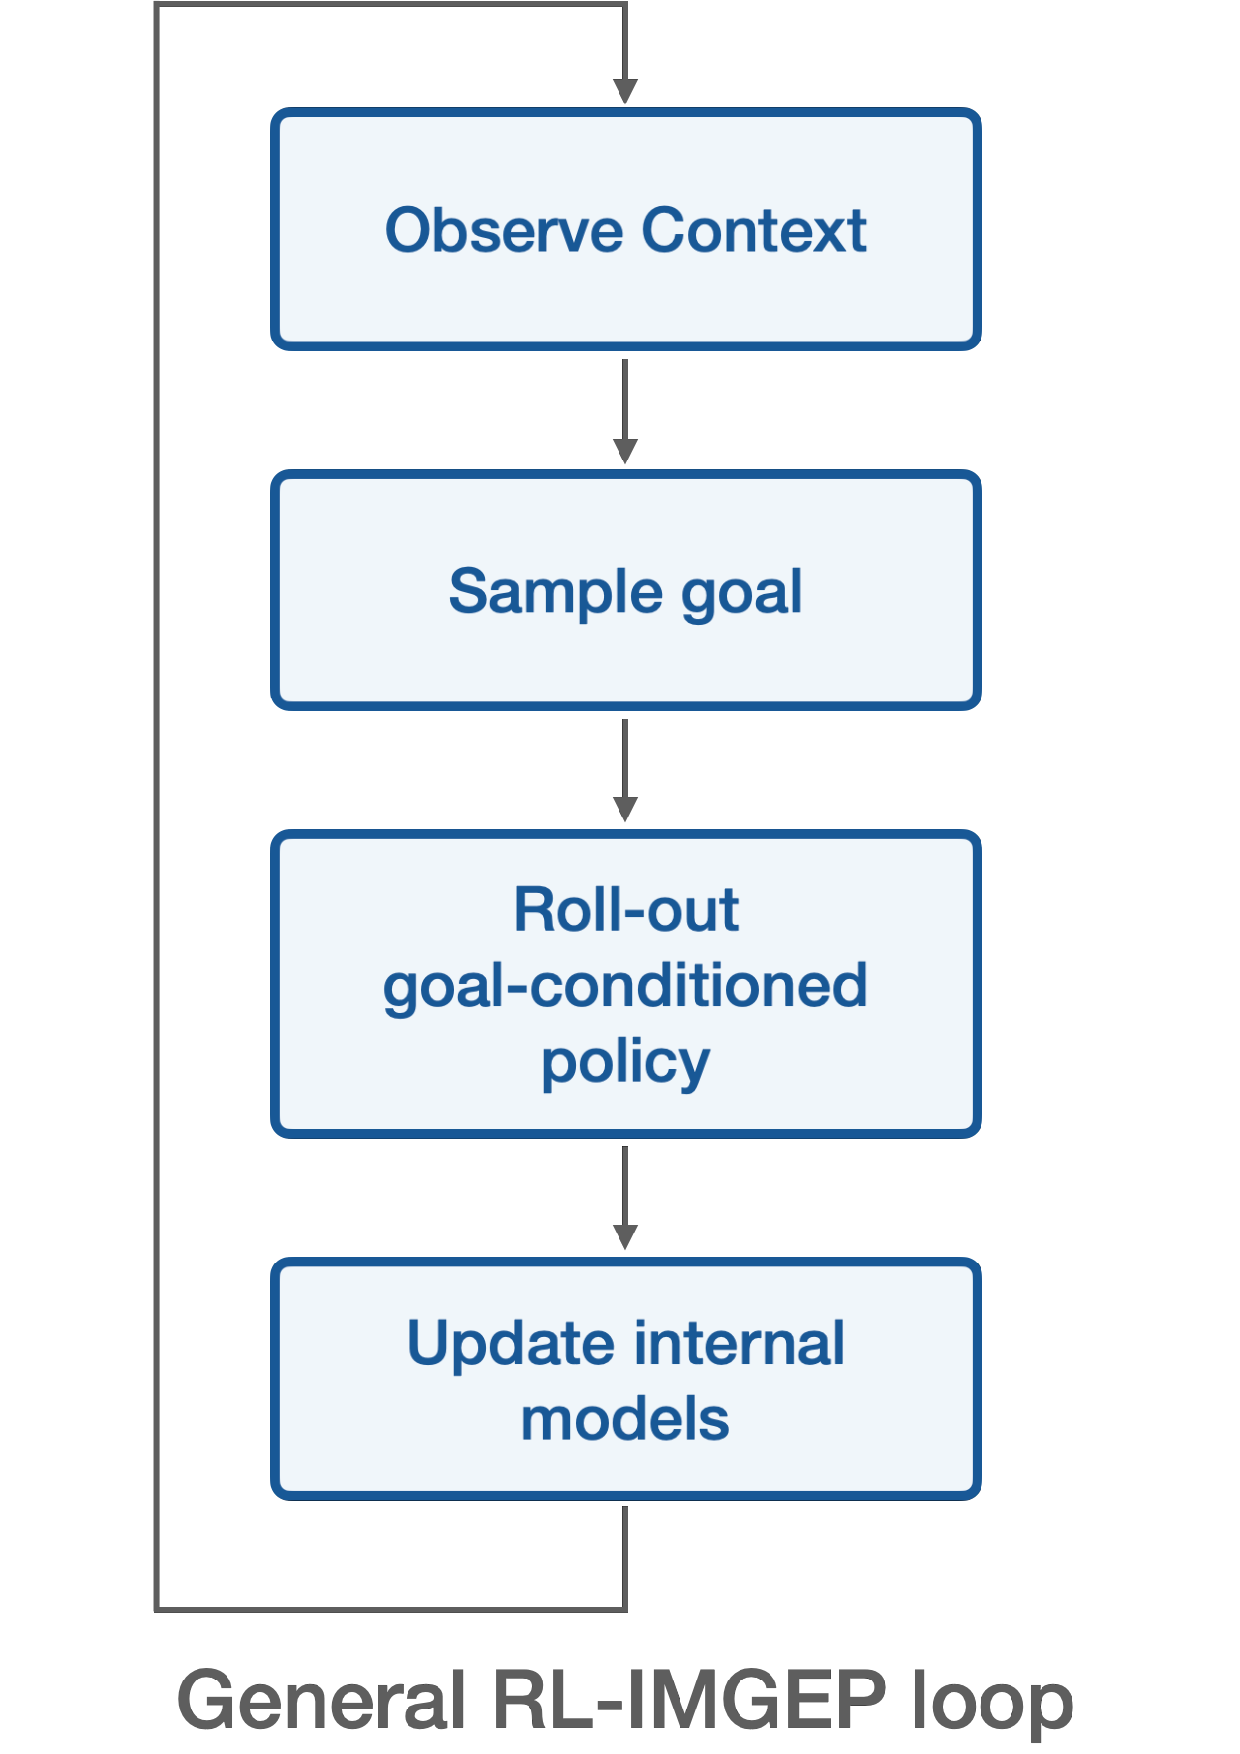
\includegraphics[width=0.9\textwidth]{survey/loop-algo.pdf}
    \end{minipage}
   \label{fig:test}
\end{minipage}
    


\subsection{A Typology of Goal Representations in the Literature}
\label{sec:survey_goal_rep}

Now that we defined the problem of interest and the overall framework to tackle it, we can start reviewing relevant approaches from the literature and how they fit in this framework. This section presents a typology of the different kinds of goal representations found in the literature. Each goal is represented by a pair: 1) a \textit{goal embedding} and 2) a goal-conditioned reward function. Figure~\ref{fig:envs} also provides visuals of the main environments used by the autotelic approaches presented in this paper.

\paragraph{Goals as Choices Between Multiple Objectives}
Goals can be expressed as a list of different objectives the agent can choose from.

\textbf{Goal embedding.} In that case, goal embeddings $z_g$ are one-hot encodings of the current objective being pursued among the $N$ objectives available. $z_g^i$ is the $i^\text{th}$ one-hot vector: $z_g^i\,=\,(\mathbbm{1}_{j=i})_{j=[1..N]}$. This is the case in \cite{oh2017zero,mankowitz2018unicorn,codevilla2018end}.

\textbf{Reward function.} The goal-conditioned reward function is a collection of $N$ distinct reward functions $R_\m{G}(\cdot)=R_i(\cdot)$ if $z_g=z_g^i$. In \cite{mankowitz2018unicorn} and \cite{chan2019actrce}, each reward function gives a positive reward when the agent reaches the corresponding object: reaching guitars and keys in the first case, monsters and torches in the second.

\paragraph{Goals as Target Features of States}
Goals can be expressed as target features of the state the agent desires to achieve.

\textbf{Goal embedding.} In this scenario, a state representation function $\varphi$ maps the state space to an embedding space $\m{Z}=\varphi(\m{S})$. Goal embeddings $z_g$ are target points in $\m{Z}$ that the agent should reach. In manipulation tasks, $z_g$ can be target block coordinates \cite{andrychowicz2017hindsight,nair2017overcoming,plappert2018multi,curious,fournier2019clic,blaes2019control,lanier2019curiosity,ding_imitation_2019,li2019towards}. In navigation tasks, $z_g$ can be target agent positions \cite<\eg in mazes, >{schaul2015universal,goalgan}. Agent can also target image-based goals. In that case, the state representation function $\varphi$ is usually implemented by a generative model trained on experienced image-based states and goal embeddings can be sampled from the generative model or encoded from real images \cite{zhu2017target,codevilla2018end,nair2018visual,pong2019skew,warde2018unsupervised,florensa2019selfsupervised,venkattaramanujam2019self,pmlr-v100-lynch20a,lynch2020grounding,nair2020contextual,kovac2020grimgep}.

\textbf{Reward function.} For this type of goals, the reward function $R_\m{G}$ is based on a distance metric $D$. One can define a dense reward as inversely proportional to the distance between features of the current state and the target goal embedding: $R_g=R_\m{G}(s|z_g)=-\alpha\times D(\varphi(s),~z_g)$ \cite<e.g. >{nair2018visual}. The reward can also be sparse: positive whenever that distance falls below a pre-defined threshold: $R_\m{G}(s|z_g)\,=\,1~\text{if}~D(\varphi(s),\,z_g)<\epsilon$, $0$ otherwise.

\paragraph{Goals as Abstract Binary Problems}
Some goals cannot be expressed as target state features but can be represented by \textit{binary problems}, where each goal expresses as set of constraint on the state (or trajectory) such that these constraints are either verified or not (binary goal achievement).

\textbf{Goal embeddings.} In binary problems, goal embeddings can be any expression of the set of constraints
that the state should respect. \cite{akakzia2020decstr,ecoffet2020first} both propose a pre-defined discrete state representation. These representations lie in a finite embedding space so that goal completion can be asserted when the current embedding $\varphi(s)$ equals the goal embedding $z_g$. Another way to express sets of constraints is via language-based predicates. A sentence describes the constraints expressed by the goal and the state or trajectory
either verifies them, or does not \cite{Hermann2017,chan2019actrce,Jiang2019,bahdanau2018learning,bahdanau2018systematic,hill2019emergent,ther,imagine,lynch2020grounding}, see \cite{Luketina2019} for a recent review. Language can easily characterize \textit{generic goals} such as ``\textit{grow any blue object}'' \cite{imagine}, \textit{relational goals} like ``\textit{sort objects by size}" \cite{Jiang2019}, ``\textit{put the cylinder in the drawer}" \cite{lynch2020grounding} or even \textit{sequential goals} ``\textit{Open the yellow door after you open a purple door}'' \cite{chevalier-boisvert2018babyai}. When goals can be expressed by language sentences, goal embeddings $z_g$ are usually language embeddings learned jointly with either the policy or the reward function. Note that, although \rl goals always express constraints on the state, we can imagine \textit{time-extended goals} where constraints are expressed on the trajectory (see a discussion in Section~\ref{sec:future_diversity}).

\textbf{Reward function.} The reward function of a binary problem can be viewed as a binary classifier that evaluates whether state $s$ (or trajectory $\tau$) verifies the constraints expressed by the goal semantics (positive reward) or not (null reward). This binary classification setting has directly been implemented as a way to learn language-based goal-conditioned reward functions $R_g(s\mid z_g)$ in \cite{bahdanau2018learning} and \cite{imagine}. Alternatively, the setup described in \cite{colas2020language} proposes to turn binary problems expressed by language-based goals into goals as specific target features. To this end, they train a language-conditioned goal generator that produces specific target features verifying constraints expressed by the binary problem. As a result, this setup can use a distance-based metric to evaluate the fulfillment of a binary goal.

\paragraph{Goals as a Multi-Objective Balance}
Some goals can be expressed, not as desired regions of the state or trajectory space but as more general objectives that the agent should maximize. In that case, goals can parameterize a particular mixture of multiple objectives that the agent should maximize.

\textbf{Goal embeddings.} Here, goal embeddings are simply sets of weights balancing the different objectives $z_g\,=\,(\beta_i)_{i=[1..N]}$ where $\beta_i$ is the weights applied to objective $i$ and $N$ is the number of objectives. Note that, when $\beta_j\,=\,1$ and $\beta_i\,=v0,~\forall i\neq j$, the agent can decide to pursue any of the objective alone. In \textit{Never Give Up}, for example, \rl agents are trained to maximize a mixture of extrinsic and intrinsic rewards \cite{badia2020never}. The agent can select the mixing parameter $\beta$ that can be viewed as a goal. Building on this approach, \textsc{agent$_{57}$} adds a control of the discount factor, effectively controlling the rate at which rewards are discounted as time goes by \cite{badia2020agent57}.

\textbf{Reward function.} When goals are represented as a balance between multiple objectives, the associated reward function cannot be represented neither as a distance metric, nor as a binary classifier. Instead, the agent needs to maximize a convex combination of the objectives: $R_g(s)\,=\,\sum_{i=1}^N~\beta_g^i R^i(s)$ where $R^i$ is the $i^\text{th}$ of $N$ objectives and $z_g=\beta=\beta_i^g\mid_{i\in[1..N]}$ is the set of weights.

%\subsection{Goal-Conditioning}
%Now that we described the different types of goal embeddings found in the literature, remains the question of how to condition the agent's behavior\,---\,\ie the policy\,---\,on them. Originally, the \uvfa framework proposed to concatenate the goal embedding to the state representation to form the policy input. Recently, other mechanisms have emerged. When language-based goals were introduced, \cite{chaplot2017gatedattention} proposed the \textit{gated-attention} mechanism where the state features are linearly scaled by attention coefficients computed from the goal representation $\varphi(z_g)$: $\text{input}\,=\,s\,\odot\,\varphi(z_g)$, where $\odot$ is the Hadamard product. Later, the Feature-wise Linear Modulation (\textsc{film}) approach \cite{perez2018film} generalized this principle to affine transformations: $\text{input}\,=\,s\,\odot\,\varphi(z_g)\, +\,\psi(z_g)$. Alternatively, \cite{Andreas_2016} came up with \textit{Neural Module Networks}, a mechanism that leverages the linguistic structure of goals to derive a symbolic program that defines how states should be processed \cite{bahdanau2018learning}.

\paragraph{Conclusion}
This section presented a diversity of goal representations, corresponding to a diversity of reward functions architectures. However, we believe this represents only a small fraction of the diversity of goal types that humans pursue. Section~\ref{sec:future} discusses other goal representations that \rl algorithms could target.

\begin{figure}[h]
    \centering
    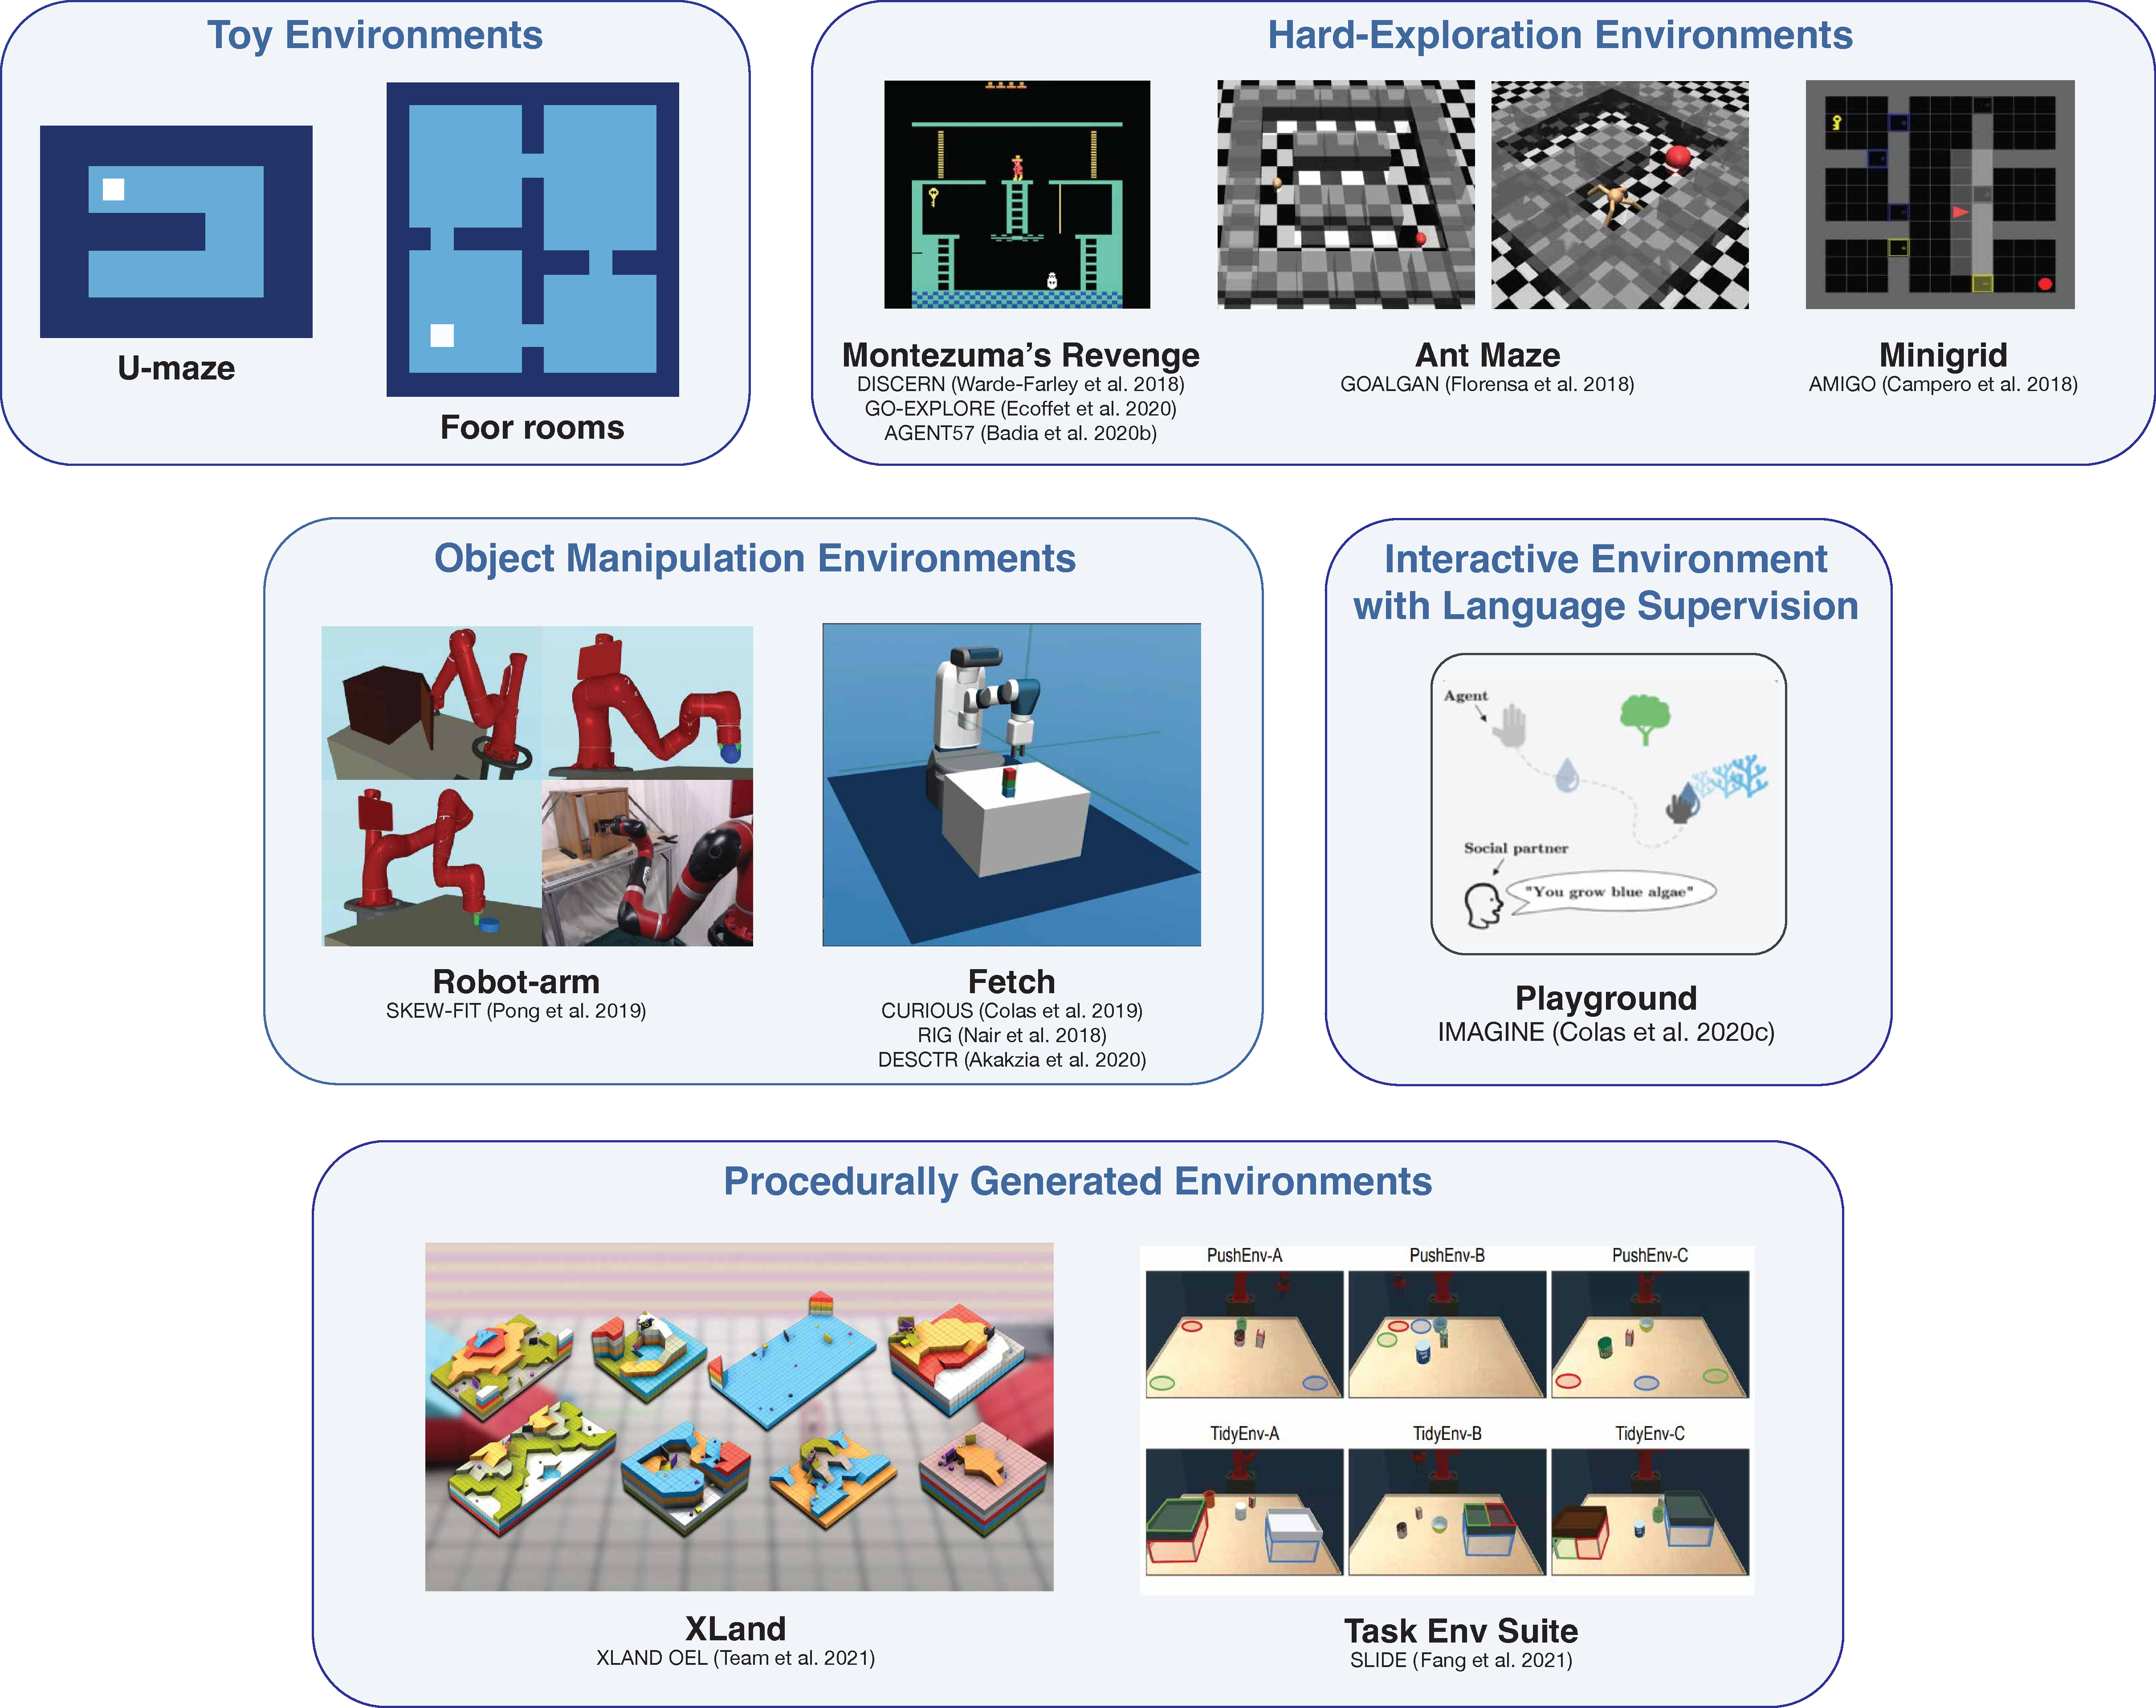
\includegraphics[width=\textwidth]{survey/survey-envs.pdf}
    \caption{\textbf{Examples of environments in autotelic RL approaches.} We organize them by dominant feature but they might share features from other catagories as well. \textit{Toy Envs.} are used to investigate and visualise goal-as-state coverage over 2D worlds; \textit{Hard-Exploration Envs.} are used to benchmark goal generation algorithms; \textit{Object Manipulation Envs.} allow for the study of the diversity of learned goals as well as curriculum learning; \textit{Interactive Envs} permit to represent goals using language and to model interaction with caregivers; \textit{Procedurally Generated Envs.} enhance the vastness of potentially reachable goals.}
    \label{fig:envs}
\end{figure}

\subsection{How to Learn Goal Representations?}
\label{sec:survey_learning_goal_rep}

The previous section discussed various types of goal representations. Autotelic agents actually need to learn these goal representations. While individual goals are represented by their embeddings and associated reward functions, representing multiple goals also requires the representation of the \textit{support} of the goal space, \ie how to represent the collection of \textit{valid goals} that the agent can sample from, see Figure~\ref{fig:goal_directed_rl}. This section reviews different approaches from the literature.

\paragraph{Assuming Pre-Defined Goal Representation}
Most approaches tackle the multi-goal \rl problem, where goal spaces and associated rewards are pre-defined by the engineer and are part of the task definition. Navigation and manipulation tasks, for example, pre-define goal spaces (\eg target agent position and target block positions respectively) and use the Euclidean distance to compute rewards \cite{schaul2015universal,andrychowicz2017hindsight,nair2017overcoming,plappert2018multi,goalgan,curious,blaes2019control,lanier2019curiosity,ding_imitation_2019,li2019towards}. \cite{akakzia2020decstr,ecoffet2020first} hand-define abstract state representation and provide positive rewards when these match target goal representations. Finally, \cite{team2021open} hand-define a large combinatorial goal space, where goals are Boolean formulas of predicates such as \textit{being near, on, seeing,} and \textit{holding}, as well as their negations, with arguments taken as entities such as \textit{objects, players}, and \textit{floors} in procedurally-generated multi-player worlds.
In all these works, goals can only be sampled from a pre-defined bounded space. This falls short of solving the intrinsically motivated skills acquisition problem. The next sub-section investigates how goal representations can be learned.

\paragraph{Learning Goal Embeddings}
Some approaches assume the pre-existence of a goal-conditioned reward function, but learn to represent goals by learning goal embeddings. This is the case of language-based approaches, which receive rewards from the environment (thus are \rlemgep), but learn goal embeddings jointly with the policy during policy learning \cite{Hermann2017,chan2019actrce,Jiang2019,bahdanau2018systematic,hill2019emergent,ther,lynch2020grounding}. When goals are target images, goal embeddings can be learned via generative models of states, assuming the reward to be a fixed distance metric computed in the embedding space \cite{nair2018visual,florensa2019selfsupervised,pong2019skew,nair2020contextual}.

\paragraph{Learning the Reward Function}
\label{sec:survey_learning_goal_rep_rew}

A few approaches go even further and learn their own goal-conditioned reward function. \cite{bahdanau2018learning,imagine} learn language-conditioned reward functions from an expert dataset or from language descriptions of autonomous exploratory trajectories respectively. However, the \textsc{agile} approach from \cite{bahdanau2018learning} does not generate its own goals.

In the domain of image-based goals, \cite{venkattaramanujam2019self,hartikainen2019dynamical} learn a distance metric estimating the square root of the number of steps required to move from any state $s_1$ to any $s_2$ and generates internal signals to reward agents for getting closer to their target goals. \cite{warde2018unsupervised} learn a similarity metric in the space of controllable aspects of the environment that is based on a mutual information objective between the state and the goal state $s_g$.

\cite{wu2018laplacian} compute a distance metric representing the ability of the agent to reach one state from another using the Laplacian of the transition dynamics graph, where nodes are states and edges are actions. More precisely, they use the eigenvectors of the Laplacian matrix of the graph given by the states of the environment as basis to compute the L2 distance towards a goal configuration.

Another way to learn reward function and their associated skills is via \textit{empowerment} methods \cite{mohamed_variational_2015,gregor2016variational,achiam_variational_2018,eysenbach2018diversity,dai_empowerment-based_2020,sharma_dynamics-aware_2020,choi_variational_2021}. Empowerment methods aim at maximizing the mutual information between the agent's actions or goals and its experienced states. Recent methods train agents to develop a set of skills leading to maximally different areas of the state space. Agents are rewarded for experiencing states that are easy to discriminate, while a discriminator is trained to better infer the skill $z_g$ from the visited states. This discriminator acts as a skill-specific reward function. 

All these methods set their own goals and learn their own goal-conditioned reward function. For these reasons, they can be considered as complete autotelic \rl algorithms.

\paragraph{Learning the Support of the Goal Distribution}
The previous sections reviewed several approaches to learn goal embeddings and reward functions. To represent collections of goals, one also needs to represent the support of the goal distribution\,---\,which embeddings correspond to valid goals and which do not.

Most approaches consider a pre-defined, bounded goal space in which any point is a valid goal (\eg target positions within the boundaries of a maze, target block positions within the gripper's reach) \cite{schaul2015universal,andrychowicz2017hindsight,nair2017overcoming,plappert2018multi,curious,blaes2019control,lanier2019curiosity,ding_imitation_2019,li2019towards}. However, not all approaches assume pre-defined goal spaces. 

The \textit{option framework} \cite{sutton_between_1999,precup_temporal_2000} proposes to train a high-level policy to compose sequences of behaviors originating from learned low-level policies called \textit{options}. Each option can be seen as a goal-directed policy where the goal embedding is represented by its index in the set of options. When options are policies aiming at specific states, \textit{option discovery} methods learn the support of the goal space; they learn which goal--state are most useful to organize higher-level behaviors. \textit{Bottleneck states} are often targeted as good sub-goals. \cite{mcgovern_automatic_2001} propose to detect states that are common to multiple successful trajectories. \cite{simsek_using_2004} propose to select state with maximal relative novelty, i.e. when the average novelty of following states is higher than the average novelty of previous ones. \cite{simsek_skill_2008} propose to leverage measures from graph theory.

The option-critic framework then opened the way to a wealth of new approaches \cite{bacon2017option}. Among those, methods based on \textit{successor features} \cite{NIPS2017_350db081,barreto2020fast,ramesh_successor_2019} propose to learn the option space using reward embeddings. With successor features, the Q-value of a goal can be expressed as a linear combination of learned reward features, efficiently decoupling the rewards from the environmental dynamics. In a multi-goal setting, these methods pair each goal with a reward embedding and use \textit{generalized policy improvement} to train a set of policies that efficiently share relevant reward features across goals. These methods provide key mechanisms to learn to discover and represent sub-goals. However, they do not belong to the \rlimgep family since high-level goals are externally provided.

Some approaches use the set of previously experienced representations to form the support of the goal distribution \cite{veeriah2018many,akakzia2020decstr,ecoffet2020first}. In \cite{goalgan}, a Generative Adversarial Network (\gan) is trained on past representations of states ($\varphi(s)$) to model a distribution of goals and thus its support. In the same vein, approaches handling image-based goals usually train a generative model of image states based on Variational Auto-Encoders (\vae) to model goal distributions and support \cite{nair2018visual,pong2019skew,nair2020contextual}. In both cases, valid goals are the one generated by the generative model.

We saw that the support of valid goals can be pre-defined, a simple set of past representations or approximated by a generative model trained on these. In all cases, the agent can only sample goals \textit{within} the convex hull of previously encountered goals (in representation space). We say that goals are \textit{within} training distribution. This drastically limits exploration and the discovery of new behaviors.

Children, on the other hand, can imagine creative goals. Pursuing these goals is thought to be the main driver of exploratory play in children \cite{chu2020exploratory}. This is made possible by the compositionality of language, where sentences can easily be combined to generate new ones. The \imagine algorithm leverages the creative power of language to generate such \textit{out-of-distribution} goals \cite{imagine}. The support of valid goals is extended to any combination of language-based goals experienced during training. They show that this mechanism augments the generalization and exploration abilities of learning agents.

In Section~\ref{sec:survey_generation}, we discuss how agents can learn to adapt the goal sampling distribution
to maximize the learning progress of the agent.

\paragraph{Conclusion}
This section presented how previous approaches tackled the problem of learning goal representations. While most approaches rely on pre-defined goal embeddings and/or reward functions, some approaches proposed to learn internal reward functions and goal embeddings jointly.

% % % % % % % % % % % % % % % % % % % % % % % % % % %
% How to generate goals?
% % % % % % % % % % % % % % % % % % % % % % % % % % % 


\subsection{How to Prioritize Goal Selection?}
\label{sec:survey_generation}

Autotelic agents also need to select their own goals. While goals can be generated by uninformed sampling of the goal space, agents can benefit from mechanisms optimizing goal selection. In practice, this boils down to the automatic adaptation of the goal sampling distribution as a function of the agent performance.

\paragraph{Automatic Curriculum Learning for Goal Selection}
In real-world scenarios, goal spaces can be too large for the agent to master all goals in its lifetime. Some goals might be trivial, others impossible. Some goals might be reached by chance sometimes, although the agent cannot make any progress on them. Some goals might be reachable only after the agent mastered more basic skills. For all these reasons, it is important to endow autotelic agents learning in open-ended scenarios with the ability to optimize their goal selection mechanism. This ability is a particular case of \textit{automatic curriculum learning} \textsc{acl} applied for goal selection: mechanisms that organize goal sampling so as to maximize the long-term performance improvement (distal objective). As this objective is usually not directly differentiable, curriculum learning techniques usually rely on a proximal objective. In this section, we look at various proximal objectives used in automatic curriculum learning strategies to organize goal selection. Interested readers can refer to \cite{portelas2020automatic}, which present a broader review of \textsc{acl} methods for \rl. Note that knowledge-based \ims can rely on similar proxies but focus on the optimization of the experienced states instead of on the selection of goals (\eg maximize next-state prediction errors). A recent review of knowledge-based \im approaches can be found in \cite{linke2019adapting}.


\paragraph{Intermediate or uniform difficulty.} Intermediate difficulty has been used as a proxy for long-term performance improvement, following the intuition that focusing on goals of intermediate difficulty results in short-term learning progress that will eventually turn into long-term performance increase. \textsc{goalgan} assigns feasibility scores to goals as the proportion of time the agents successfully reaches it \cite{goalgan}. Based on this data, a \gan is trained to generate goals of intermediate difficulty, whose feasibility scores are contained within an intermediate range. \cite{sukhbaatar2017intrinsic} and \cite{campero2020learning} train a goal policy with \rl to propose challenging goals to the \rl agent. The goal policy is rewarded for setting goals that are neither too easy nor impossible. In the same spirit, \cite{team2021open} use a mixture of three criteria to filter valid goals: 1) the agent has a low probability of scoring high; 2) the agent has a high probability of scoring higher than a control policy; 3) the control policy performs poorly. Finally, \cite{zhang2020automatic} select goals that maximize the disagreement in an ensemble of value functions. Value functions agree when the goals are too easy (the agent is always successful) or too hard (the agent always fails) but disagree for goals of intermediate difficulty.

\cite{settersolver} propose a variant of the \textsc{goalgan} approach and train a goal generator to sample goals of all levels of difficulty, uniformly. This approach seems to lead to better stability and improved performance on more complex tasks compared to \textsc{goalgan} \cite{goalgan}.

Note that measures of intermediate difficulty are sensitive to the presence of stochasticity in the environment. Indeed, goals of intermediate difficulty can be detected as such either because the agent has not yet mastered them, or because the environment makes them impossible to achieve sometimes. In the second case, the agent should not focus on them, because it cannot learn anything new. Estimating medium-term learning progress helps overcoming this problem (see below).
 
 
\paragraph{Novelty - diversity.}  \cite{warde2018unsupervised,pong2019skew,pitis2020maximum} all bias the selection of goals towards sparse areas of the goal space. For this purpose, they train density models in the goal space. While \cite{warde2018unsupervised,pong2019skew} aim at a uniform coverage of the goal space (diversity), \cite{pitis2020maximum} skew the distribution of selected goals even more, effectively maximizing novelty. \cite{kovac2020grimgep} proposed to enhance these methods with a goal sampling prior focusing goal selection towards controllable areas of the goal space. Finally, \cite{Fang-RSS-21} use procedural content generation (\textsc{pcg}) to train a task generator that produces diverse environments in which agents can explore customized skills. 

These algorithms have strong connections with empowerment methods \cite{mohamed_variational_2015,gregor2016variational,achiam_variational_2018,eysenbach2018diversity,campos_explore_2020,sharma_dynamics-aware_2020,choi_variational_2021}. Indeed, the mutual information between goals and states that empowerment methods aim to maximize can be rewritten as: 
\begin{equation*}
    I(Z,\,S) = H(Z) - H(Z\mid S).
\end{equation*}
Thus, maximizing empowerment can be seen as maximizing the entropy of the goal distribution while minimizing the entropy of goals given experienced states. Algorithm that both learn to sample diverse goals $(H(Z)\nearrow)$ and learn to represent goals with variational auto-encoders $(H(Z|S)\searrow)$ can be seen as maximizing empowerment. The recent wealth of \textit{empowerment} methods, however, rarely discusses the link with autotelic agents: they do not mention the notion of goals or goal-conditioned reward functions and do not discuss the problem of goal representations \cite{gregor2016variational,achiam_variational_2018,eysenbach2018diversity,campos_explore_2020,sharma_dynamics-aware_2020}. In a recent paper, \cite{choi_variational_2021} investigated these links and formalized a continuum of methods from empowerment to visual goal-conditioned approaches. 

While \textit{novelty} refers to the \textit{originality} of a reached outcome, \textit{diversity} is a term that can only be applied to a collection of these outcomes. An outcome will be said novel if it is semantically different from what exists in the set of known outcomes. A set of outcomes will be said \textit{diverse} when outcomes are far from each other and \textit{cover well} the space of possible outcomes. Note that agents can also express diversity in their behavior towards a unique outcome, a skill known as \textit{versatility} \cite{hausman_learning_2018,kumar_one_2020,osa_discovering_2021,celik_specializing_2021}.

\paragraph{Medium-term learning progress.} 
The idea of using learning progress (\lp) as a intrinsic motivation for artificial agents dates back to the 1990s \cite{schmidhuber1991curious,schmidhuber1991learning,kaplan_maximizing_2004,oudeyer_intrinsic_2007}. At that time, however, it was used as a knowledge-based \im and rewarded progress in predictions. From 2007, \cite{oudeyer2007intrinsic} suggested to use it as a competence-based \im to reward progress in competence instead. In such approaches, agents estimate their \lp in different regions of the goal space and bias goal sampling towards areas of high absolute learning progress using bandit algorithms \cite{baranes2013active,moulinfriergmm,forestier2016modular,fournier2018accuracy,fournier2019clic,curious,blaes2019control,portelas_teacher_2020,akakzia2020decstr}. Such estimations attempts to disambiguate the incompetency or uncertainty the agent could resolve with more practice (epistemic) from the one it could not (aleatoric). Agents should indeed focus on goals towards which they can make progress and avoid goals that are either too easy, currently too hard, or impossible. 

\cite{forestier2016modular,curious,blaes2019control} and \cite{akakzia2020decstr} organize goals into modules and compute average \lp measures over modules. \cite{fournier2018accuracy} defines goals as a discrete set of precision requirements in a reaching task and computes \lp for each requirement value. The use of absolute \lp enables agents to focus back on goals for which performance decreases (due to perturbations or forgetting). \cite{akakzia2020decstr} introduces the success rate in the value optimized by the bandit: $v\,=\,(1\,-\,\text{\textsc{sr}})\,\times\,\text{\textsc{lp}}$, so that agents favor goals with high absolute \lp and low competence.

\paragraph{Hierarchical Reinforcement Learning for Goal Sequencing.}

Hierarchical reinforcement learning (\hrl) can be used to guide the sequencing of goals \cite{dayan1993feudal,sutton1998intra,sutton_between_1999,precup2001temporal}. In \hrl, a high-level policy is trained via \rl or planning to generate sequence of goals for a lower level policy so as to maximize a higher-level reward. This allows to decompose tasks with long-term dependencies into simpler sub-tasks. Low-level policies are implemented by traditional goal-conditioned \rl algorithms \cite{levy2018hierarchical,roder2020curious} and can be trained independently from the high-level policy \cite{kulkarni2016hierarchical,frans2017meta} or jointly \cite{levy2018hierarchical,nachum2018data,roder2020curious}. In the option framework, option can be seen as goal-directed policies that the high-level policy can choose from~\cite{sutton_between_1999,precup_temporal_2000}. In that case, goal embeddings are simple indicators. Most approaches consider hand-defined spaces for the sub-goals (\eg positions in a maze). Recent approaches propose to use the state space directly \cite{nachum2018data} or to learn the sub-goal space (e.g. \cite{vezhnevets2017feudal}, or with generative model of image states in  \cite{nasiriany2019planning}). 




%\subsection{Language as a Tool for Creative Goal Generation}
%\label{sec:future_language_goals}
%Whether they are specific or abstract, time-specific or time-extended, whether they represent mixture of objectives, constraints, or logical combinations, all goals can be expressed easily by humans through language. Language, thus, seems like the ideal candidate to express goals in \rl agents. So far, language was only used to formulate a few forms of goals (see Section~\ref{sec:survey_goal_rep}). In the future, it might be used to express any type of goals. Recurrent Neural Networks (\rnn) \cite{elman}, Deep Sets \cite{deepset}, Graph Neural Networks (\gnn) or Transformers are all architectures that benefits from inductive biases and could be leveraged to facilitate new forms of goal representations (time-extended, set-based, relational etc.). As a learning signal, \cite{imagine} propose to leverage descriptive sentences from social partners as a way to train goal representations. Mixing self-supervised learning and language inputs from humans as in \cite{lynch2020grounding} might be the way forward. 


% % % % % % % % % % % % % % % % % % % % % % % % % % %
% Discussion \& Conclusion
% % % % % % % % % % % % % % % % % % % % % % % % % % % 
\subsection{Discussion \& Conclusion}

This paper defined the intrinsically motivated skills acquisition problem and proposed to view autotelic \rl algorithms or \rlimgep as computational tools to tackle it. These methods belong to the new field of \textit{developmental reinforcement learning}, the intersection of the developmental robotics and \rl fields. We reviewed current goal-conditioned \rl approaches under the lens of autotelic agents that learn to represent and generate their own goals in addition of learning to achieve them.

We propose a new general definition of the \textit{goal} construct: a pair of compact goal representation and an associated goal-achievement function. Interestingly, this viewpoint allowed us to categorize some \rl approaches as goal-conditioned, even though the original papers did not explicitly acknowledge it. For instance, we view the Never Give Up \cite{badia2020never} and Agent 57 \cite{badia2020agent57} architectures as goal-conditioned, because agents actively select parameters affecting the task at hand (parameter mixing extrinsic and intrinsic objectives, discount factor) and see their behavior affected by this choice (goal-conditioned policies).

This point of view also offers a direction for future research. Autotelic agents need to learn to represent goals and to measure goal achievement. Future research could extend the diversity of considered goal representations, investigate novel reward function architectures and inductive biases to allow time-extended goals, goal composition and to improve generalization.

%\todo{Maybe discuss the link with the GVF from Sutton and his question/answer stuff}\\
The general vision we convey in this paper builds on the metaphor of the learning agent as a curious scientist. A scientist that would formulate hypotheses about the world and explore it to find out whether they are true. A scientist that would ask questions, and setup intermediate goals to explore the world and find answers. A scientist that would set challenges to itself to learn about the world, to discover new ways to interact with it and to grow its collection of skills and knowledge. Such a scientist could decide of its own agenda. It would not need to be instructed and could be guided only by its curiosity, by its desire to discover new information and to master new skills. Autotelic agents should nonetheless be immersed in complex socio-cultural environment, just like humans are. In contact with humans, they could learn to represent goals that humans and society care about. 

\clearpage
%\begin{landscape}
%\end{landscape}
\begin{landscape}
\begin{table*}[t!]
\tiny
\centering

\begin{tabular}{l|cccc}
\hline
\multirow{2}{*}{\textbf{Approach}} & \multirow{2}{*}{\textbf{Goal Type}} & \multirow{2}{*}{\textbf{\shortstack{Goal \\ Rep.}}} & \multirow{2}{*}{\textbf{\shortstack{Reward\\ Function}}} & \multirow{2}{*}{\textbf{\shortstack{Goal sampling \\ strategy}}} \\
\\
\hline
\multicolumn{5}{l}{\textbf{RL-IMGEPs that assume goal embeddings and reward functions}}\\
\hline
\cite{fournier2018accuracy} & Target features (+tolerance) & Pre-def & Pre-def & \lp-Based\\
\textsc{hac} \cite{levy2018hierarchical} & Target features & Pre-def & Pre-def & \hrl \\
\textsc{hiro} \cite{nachum2018data} & Target features & Pre-def & Pre-def & \hrl \\
\textbf{CURIOUS} \cite{curious} & Target features & Pre-def & Pre-def & \lp-based\\
\textbf{CLIC} \cite{fournier2019clic} & Target features & Pre-def & Pre-def & \lp-based\\
\textbf{CWYC} \cite{blaes2019control} & Target features & Pre-def & Pre-def & \lp-based + surprise\\
\textsc{go-explore} \cite{ecoffet2020first} & Target features & Pre-def & Pre-def & Novelty \\
\textsc{ngu} \cite{badia2020never} & Objectives balance & Pre-def & Pre-def & Uniform \\
\textsc{agent} 57 \cite{badia2020agent57} & Objectives balance & Pre-def & Pre-def & Meta-learned \\ 
\textbf{DECSTR} \cite{akakzia2020decstr} & Binary problem & Pre-def & Pre-def & \lp-based \\
\textsc{slide} \cite{Fang-RSS-21} & Skill index & Pre-def & Pre-def & Novelty (PCG)\\
\textsc{XLand OEL} \cite{team2021open} & Binary problem & Pre-def & Pre-def & Intermediate difficulty \\
\hline
\multicolumn{5}{l}{\textbf{RL-IMGEPs that learn their goal embedding and assume reward functions}}\\
\hline
%\cite{sutton2011horde} & & & & \\
\textsc{rig} \cite{nair2018visual} & Target features (images) & Learned (\vae) & Pre-def & From \vae prior \\
\textsc{goalgan} \cite{goalgan} & Target features & Pre-def + GAN & Pre-def & Intermediate difficulty\\
\cite{florensa2019selfsupervised} & Target features (images) & Learned (\vae) & Pre-def & From \vae prior \\
\textsc{skew-fit} \cite{pong2019skew} & Target features (images) & Learned (\vae) & Pre-def & Diversity \\
\textsc{setter-solver} \cite{settersolver} & Target features (images) & Learned (Gen. model) & Pre-def & Uniform difficulty \\
\textsc{mega} \cite{pitis2020maximum} & Target features (images) & Learned (\vae) & Pre-def & Novelty \\
\textsc{cc-rig} \cite{nair2020contextual} & Target features (images) & Learned (\vae)  & Pre-def & From \vae prior \\
\textsc{amigo} \cite{campero2020learning} & Target features (images) & Learned (with policy) & Pre-def  & Adversarial \\ 
\textbf{GRIMGEP} \cite{kovac2020grimgep} & Target features (images) & Learned (with policy) & Pre-def & Diversity and ALP \\
\hline
\multicolumn{5}{l}{\textbf{Full RL-IMGEPs}}\\
\hline
\textsc{discern} \cite{warde2018unsupervised} & Target features (images) & Learned (with policy) & Learned (similarity) & Diversity \\
\textsc{diayn} \cite{eysenbach2018diversity} & Discrete skills & Learned (with policy) & Learned (discriminability) & Uniform \\
\cite{hartikainen2019dynamical} & Target features (images) & Learned (with policy) & Learned (distance) & Intermediate difficulty  \\
\cite{venkattaramanujam2019self} & Target features (images) & Learned (with policy) & Learned (distance) & Intermediate difficulty \\
\textbf{IMAGINE} \cite{imagine} & Binary problem (language) & Learned (with reward) & Learned & Uniform + Diversity \\
\textsc{vgcrl} \cite{choi_variational_2021} & Target features & Learned  & Learned & Empowerment \\
\end{tabular}
\caption{
\small \textbf{A classification of autotelic RL-IMGEP approaches.} \small Autotelic approaches require agents to sample their own goals. The proposed classification groups algorithms depending on their degree of autonomy: 1) \rlimgeps that rely on pre-defined goal representations (embeddings and reward functions); 2) \rlimgeps that rely on pre-defined reward functions but learn goal embeddings and 3) \rlimgeps that learn complete goal representations (embeddings and reward functions). For each algorithm, we report the type of goals being pursued (see Section~\ref{sec:survey_goal_rep}), whether goal embeddings are learned (Section~\ref{sec:survey_learning_goal_rep}), whether reward functions are learned (Section~\ref{sec:survey_learning_goal_rep_rew}) and how goals are sampled (Section~\ref{sec:survey_generation}). We mark in bold algorithms that use a developmental approaches and explicitly pursue the intrinsically motivated skills acquisition problem.}
\label{tab:bigtable}
\end{table*}
\end{landscape}
\clearpage


\section{From Autotelic to Vygotkian Agents}

\begin{abstract} % 214 mots
Building autonomous agents able to grow open-ended repertoires of skills across their lives is a fundamental goal of artificial intelligence (\ai). A promising developmental approach recommends the design of intrinsically motivated agents that learn new skills by generating and pursuing their own goals\,---\,\textit{autotelic agents}. But despite recent progress, existing algorithms still show serious limitations in terms of goal diversity, exploration, generalization or skill composition. 
% 
This perspective calls for the immersion of autotelic agents into \textit{rich socio-cultural worlds}, an immensely important attribute of our environment that shapes human cognition but is mostly omitted in modern \ai. 
Inspired by the seminal work of Vygotsky, we propose \textit{Vygotskian autotelic agents}\,---\,agents able to internalize their interactions with others and turn them into \textit{cognitive tools}. We focus on language and show how its structure and informational content may support the development of new cognitive functions in artificial agents like it does in humans.
% 
We justify the approach by uncovering several examples of new artificial cognitive functions emerging from interactions between language and embodiment in recent works at the intersection of deep reinforcement learning and natural language processing. Looking forward, we highlight future opportunities and challenges for a Vygotskian Autotelic AI research, including the use of language models as cultural models supporting artificial cognitive development. 

\end{abstract}

\subsection*{Introduction}
%our goal
Humans are remarkable examples of lifelong open-ended learners. They learn to recognize objects and crawl as infants, learn to ask questions and interact with peers as toddlers, learn to master engineering, science, or arts as adults. A fundamental goal of artificial intelligence (\ai) is to build autonomous agents capable of growing such open-ended repertoires of skills. 

% RL and deep RL
\textit{Reinforcement learning} (\rl) offers a mathematical framework to formalize and tackle skill learning problems. For an embodied and situated \rl agent, \textit{learning a skill} (\eg playing chess) is about learning to act so as to maximize future \textit{rewards} measuring progression in that skill (\eg +1 for winning a game, -1 for losing it).\cite{sutton_introduction_1998} Extensions based on modern deep learning methods (deep \rl) have recently made the headlines by solving a wealth of problems we thought only humans could solve: beating chess and go world champions,\cite{silver2016mastering} controlling stratospheric balloons,\cite{bellemare2020autonomous} or even maintaining plasma in fusion reactors.\cite{degrave2022magnetic} But human chess world champions can also run, cook, draw a cat, or make a friend laugh. Humans are proficient in a wide diversity of tasks, most of which they just invent for themselves. The \rl framework, in its standard form, considers a single predefined reward function and, thus, must be extended (see Figure~\ref{fig:rl_arl_varl}, a).

\vspace{.4cm}

\begin{figure}[!ht]
    \centering
    \captionsetup{width=.85\linewidth}
    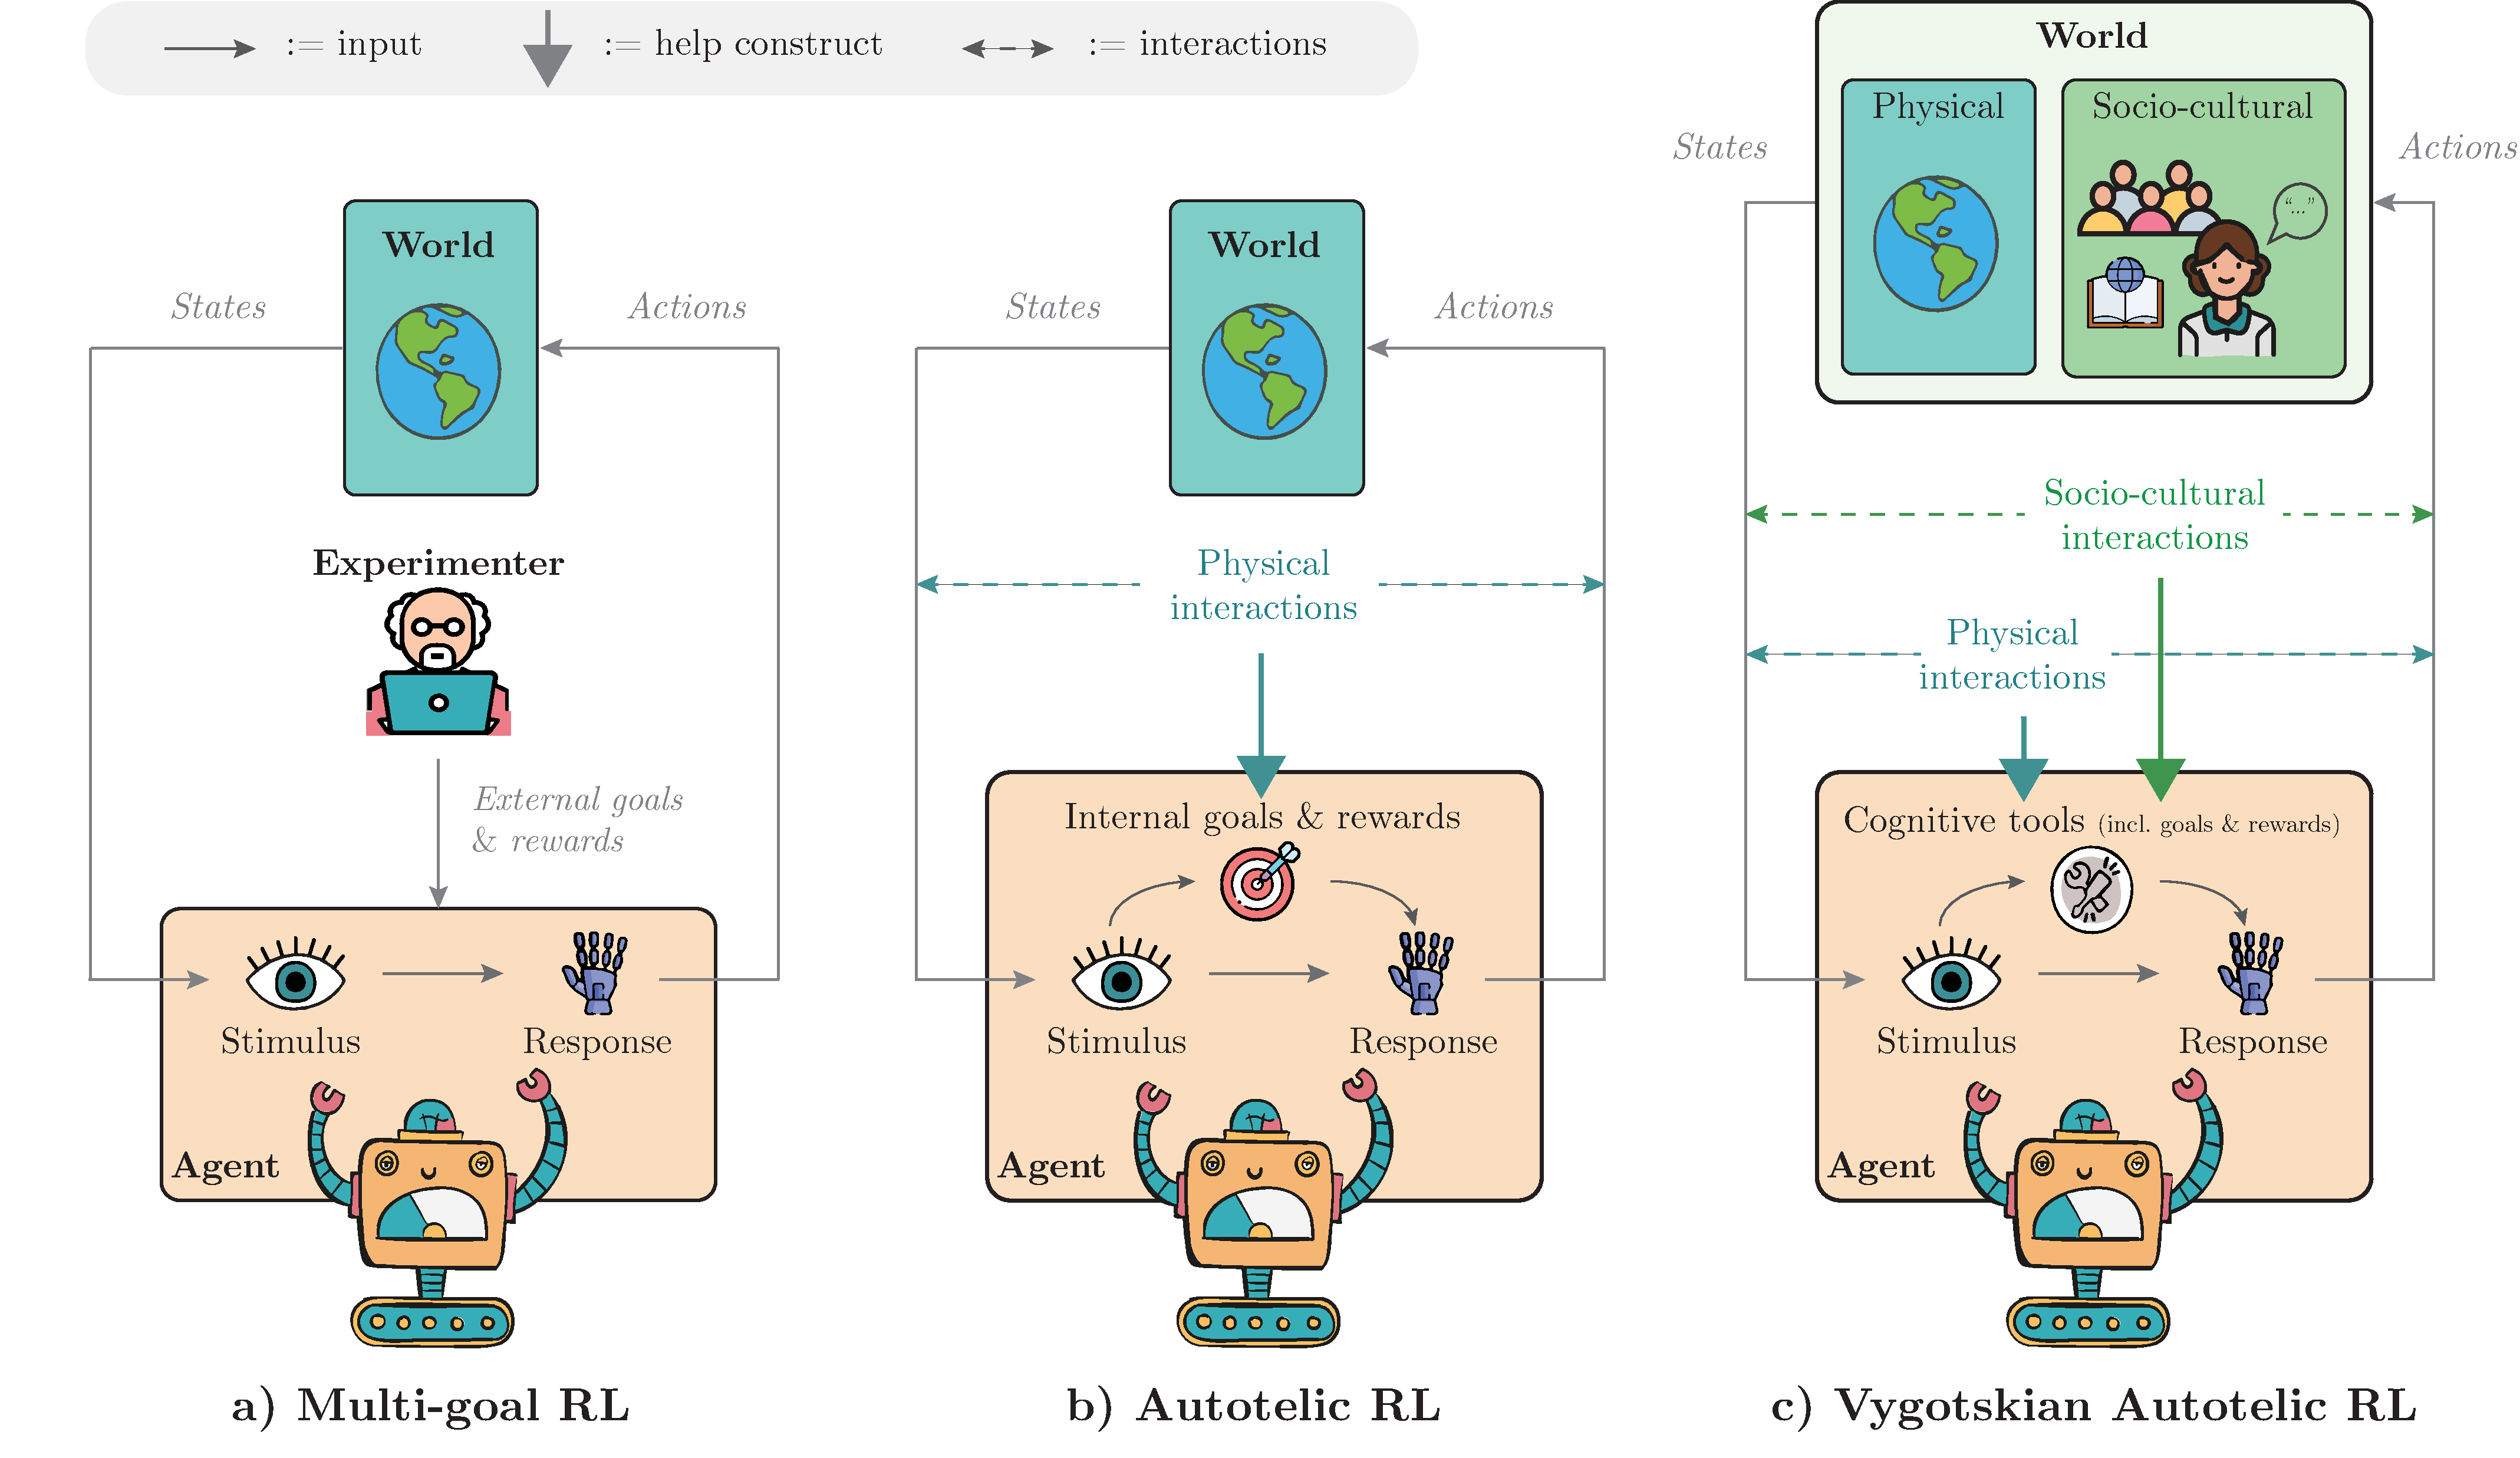
\includegraphics[width=\linewidth]{perspective/figure-intro-v4.pdf}
    \caption{\small From multi-goal RL to autotelic RL to Vygotskian autotelic RL. \rl defines an agent experiencing the state of the world as stimuli and acting on that world via actions. Multi-goal RL (a): goals and associated rewards come from pre-engineered functions and are perceived as sensory stimuli by the agent. Autotelic RL (b): agents build internal goal representations from interactions between their intrinsic motivations and their physical experience of the world (Piagetian view). Vygotskian autotelic RL (c): agents internalize physical and socio-cultural interactions into \textit{cognitive tools}. Here, \textit{cognitive tools} refer to any self-generated representation that mediates stimulus and actions. This can include self-generated goals, explanations, descriptions, attentional biases, visual aids, mnemotechnic tricks, etc. }
    \label{fig:rl_arl_varl}
\end{figure}

\vspace{.4cm}


% Piagetian view and autotelic learning
Jean Piaget, a pioneer of developmental psychology, demonstrated children's ability to set their own goals, shape their own learning trajectories, and develop in symbiosis with their physical environment.\cite{piaget1952origins} His work influenced future developments in both psychology and \ai.\cite{dautenhahn_studying_1999} Indeed, if each skill is the association of a goal (\eg ``be a good chess player'') and a policy to reach it, then \textit{open-ended skill discovery} presupposes the ability to invent and select one's own goals and reward functions so as to progressively build repertoires of skills. \textit{Autotelic \textsl{\rl}}\,---\,from the Greek \textit{auto} (self) and \textit{telos} (goal)\,---\,extends the \rl framework to build such agents.\cite{colas2021intrinsically} It integrates two extensions of the standard \rl framework: the ability to consider multiple goals in parallel (\textit{multi-goal \textsl{\rl}}) and the ability to represent and select one's own goals. Although the first extension is straightforward,\cite{schaul_universal_2015} the second requires another ingredient inspired by the study of human learning: \textit{intrinsic motivations}. 

% intrinsic motivations
Most of the human time is spent on activities that do not seem to satisfy any utilitarian end; think about children playing, or adults watching movies. Psychologists argue that such exploratory behaviors are powered by \textit{intrinsic motivations} (\im), a set of brain processes driving us to experience situations for the mere pleasure of experiencing novelty, surprise, or learning progress.\cite{berlyne_curiosity_1966,  kidd_psychology_2015, gottlieb_towards_2018}
Similar processes can be coded into artificial agents to foster spontaneous exploratory capabilities.\cite{schmidhuber_curious_1991, barto_intrinsic_2005, oudeyer_intrinsic_2007} Among them, \textit{knowledge-based \textsl{\im}} drive agents to experience parts of the environment to improve their internal models of the world and \textit{competence-based \textsl{\im}} let them improve their mastery of self-generated goals.\cite{oudeyer_what_2009} In the Piagetian tradition, autotelic agents see their goal representation and goal selection mechanisms emerge from interactions between competence-based \im and their experience of the physical world (see Figure~\ref{fig:rl_arl_varl}, b).\cite{colas2021intrinsically}

% limits of autotelic learning
In practice, current autotelic \rl implementations still lack human-like open-endedness. The goal representations emerging from their intrinsically motivated experience with the physical world end up very concrete and mostly consist in reaching target stimuli (\eg matching their visual input with a particular target).\cite{colas2021intrinsically} This contrasts with the wide diversity and the abstraction of goals targeted by humans. In addition, the generated goals very often belong to the distribution of previously experienced effects, which drastically limits the ability of autotelic agents to represent \textit{creative goals}, thus to explore and undergo an open-ended discovery process.\cite{colas_language_2020} Besides goal imagination, \rl algorithms still lack human-like capacities in terms of generalization, skill composition, abstraction, or sample efficiency.\cite{witty2021measuring,shanahan2022abstraction} 

% vygotsky and socio-cultural situatedness
The way forward might build on an alternative view of child development proposed by another pioneer of developmental psychology called Lev Vygotsky. Humans are social beings; intrinsically motivated to interact and cooperate with their peers.\cite{tomasello_cultural_1999,tomasello_understanding_2005, brewer2014addressing} For Vygotsky, linguistic social interactions such as descriptions, explanations, corrections, or play start as interpersonal processes before they are turned into \textit{intrapersonal} cognitive processes through the process of \textit{internalization}.\cite{vygotsky_thought_1934} Following his vision, many psychologists,\cite{berk_why_1994,lupyan_what_2012,gentner_analogy_2017} linguists,\cite{whorf_language_1956,rumelhart_sequential_1986,lakoff2008metaphors} and philosophers \cite{hesse1988cognitive,dennett_consciousness_1993,carruthers_magic_1998,carruthers_modularity_2002} argued for the importance of socio-cultural interactions in the development of human intelligence. 

What does this mean for \ai? We advocate for a \textit{Vygotskian Autotelic AI}. Specifically, we propose to immerse autotelic agents into our rich socio-cultural world; to let them interact with us and with their peers in natural language; to let them internalize these interactions and mesh them with their cognitive development (see Figure~\ref{fig:rl_arl_varl}, c). Just like they do for humans, language and culture will help shape the agents' goal representations and generation mechanisms, thereby offering them the ability to generate more diverse and abstract goals; to imagine new goals beyond their past experience. Because they will develop at our contact, bathed in our cultures, they will learn about our cultural norms, values, customs, interests, and thought processes; all of which would be impossible to learn in social isolation. Just like humans, machines will use language to develop higher cognitive functions like abstraction, generalization, or imagination.\cite{carruthers_language_1998, gentner_analogy_2017, dove_language_2018} As we will see, this process has already started. 

Recent advances in \ai make our proposition particularly timely. Indeed, these past years have seen a revolution in natural language processing (\nlp), the set of tools designed to analyze and generate language. Generative models of language trained on gigantic amounts of text can now produce high-quality language,\cite{brown2020language} handle multimodal inputs,\cite{radford2021learning,ramesh2022hierarchical,alayrac2022flamingo} and capture common sense\cite{west_symbolic_2021} or cultural artefacts.\cite{hershcovich_challenges_2022,arora2022probing} Pure language models like GPT-3\cite{brown2020language} are capable of impressive zero-shot generalizations including joke explanations, arithmetic, question answering, or even multi-step reasoning when nudged appropriately.\cite{creswell2022selection} Multi-modal variants can explain visual jokes (memes)\cite{alayrac2022flamingo} or generate impressive images from the most creative descriptions its testers can come up with.\cite{ramesh_zero-shot_2021,ramesh2022hierarchical} The ongoing convergence of autotelic \rl and \nlp will offer a wealth of opportunities as autotelic agents learn to interact with us, learn from us and teach us back. This motivates the elaboration of a theoretical framework to understand recent linguistic \rl developments and point towards future challenges in the quest for open-ended skill discovery.

This perspective extends previous calls to leverage Vygotsky's insights for a more socially-situated cognitive robotics.\cite{dautenhahn_studying_1999, zlatev_epigenesis_2001, lindblom_social_2003,mirolli_towards_2011} Zlatev discussed interactions between social-situatedness and epigenetic development,\cite{zlatev_epigenesis_2001} Dautenhahn and Billard drew the parallel between \ai and the Piagetian vs.\, Vygotskian views,\cite{dautenhahn_studying_1999} while Mirolli and Parisi, as well as Cangelosi et al., reviewed the first successful auxiliary uses of language for decision-making.\cite{mirolli_towards_2011, cangelosi2010integration} In the last decade however, the \ai community seems to have lost track of these insights. Today we update these arguments in the light of recent \ai advances and reframe the Vygotskian perspective within the autotelic \rl framework. As a result, we will not discuss non-embodied multi-modal supervised techniques\cite{radford2021learning, ramesh2022hierarchical, alayrac2022flamingo} or non-linguistic autotelic \rl.\cite{schaul_universal_2015} We will not cover the advances in the sub-field of \rl dedicated to the computational modeling of social interactions (social \rl).\cite{jaques2019social} Although future Vygotskian autotelic agents must incorporate social \rl mechanisms, current approaches do not consider autotelic agents able to set their own goals and, as such, do not tackle the open-ended skill discovery problem (see a complete discussion in a related paper\cite{sigaud_towards_2021}).

The next section sets the background and discusses the interaction between language and thought in humans by building on the work of psychologists and philosophers (Section~\ref{sec:4views}). The two following sections dive into the two key elements of a Vygotskian autotelic \ai identified in Section~\ref{sec:4views}: 1)~the ability to exploit information contained in linguistic structure and content (syntax, vocabulary, narratives) to support the development of cognitive functions (Section~\ref{sec:extraction}); 2)~the ability to internalize linguistic interactions within the agent to power its future autonomy and integration into the socio-cultural world (Section~\ref{sec:production}). Finally, Section~\ref{sec:challenges} identifies open challenges for future research.



% % % % % % % % % % % % % % % % % % % % % % % % % % % % % % % % % % % % % % % % % % % % 
% Section 1: Language and Thought in Humans
% % % % % % % % % % % % % % % % % % % % % % % % % % % % % % % % % % % % % % % % % % % % 
\subsection{Language and Thought in Humans, a Vygotskian Perspective}
\label{sec:language_and_though}
Our ability to generate new ideas is the source of our incredible success in the animal kingdom. But this ability did not appear with the first \textit{homo sapiens} 130,000 years ago. Indeed, the oldest imaginative artifacts such as figurative arts, elaborate burials or the first dwellings only date back to 70,000 years ago.\cite{harari_sapiens_2014, vyshedskiy_language_2019} This is thought to coincide with the apparition of \textit{recursive language}.\cite{goldberg1999emergence, vyshedskiy_language_2019, hoffmann_construction_2020} Which of these appeared first? Creativity or recursive language? Or did they mutually bootstrap?

Extreme views on the topic either characterize language as a pure communicative device to convey our inner thoughts (strong communicative thesis)\cite{chomsky_syntactic_1957,fodor1975language} or, on the other hand, argue that only language can be the vehicle of our thoughts (strong cognitive thesis)\cite{wittgenstein1953philosophical, mcdowell1996mind} As often, the truth seems to lie in between. Animal and preverbal infants demonstrate complex cognition,\cite{sperber1995causal, allen1999species} but language does impact the way we perceive,\cite{waxman_words_1995, yoshida_sound_2003} represent concepts,\cite{lakoff2008metaphors} conduct compositional and relational thinking,\cite{gentner2002relational, gentner_analogy_2017, vyshedskiy_language_2019} etc. Thus, language seems to be at least \textit{required} to develop some of our cognitive processes (requirement thesis), and might still be the vehicle of \textit{some} of our thoughts (constitutive thesis).\cite{carruthers_language_1998} Interested readers can find a thorough overview of this debate in \textit{Language and Thought} by Carruthers and Boucher.\cite{carruthers_language_1998}

If language is required to develop some of our higher cognitive functions, then autotelic artificial agents should use it as well. But how does that work? What is so special about language? 
Let us start with \textit{words}, which some called \textit{invitations to form categories}.\cite{waxman_words_1995} Hearing the same word in a variety of contexts invites humans to compare situations, find similarities, differences and build symbolic representations of agents, object and their attributes. With words, the continuous world can be simplified and structured into mental entities at various levels of abstraction. 

%The recursivity and partial compositionality of languages allow us to readily understand the meaning of sentences we never heard before by generalizing from known words and syntactic structures
The recursivity and partial compositionality of language allows us to readily understand the meaning of sentences we never heard before by generalizing from known words and syntactic structures. On the flip side, it also supports \textit{linguistic productivity},\cite{chomsky_syntactic_1957} the ability to generate new sentences\,---\,thus new ideas\,---\,in an open-ended way. 
Relational structures such as comparisons and metaphors facilitate our relational thinking,\cite{gentner2002relational, gentner_analogy_2017} condition our ability to compose mental images,\cite{vyshedskiy_language_2019} and support our understanding of abstract concepts such as emotions, politics or scientific theories.\cite{hesse1988cognitive,lakoff2008metaphors} 

Finally, language is a cultural artefact inherited from previous generations and shared with others. It supports our cultural evolution and allows humans to efficiently transfer knowledge and practices across people and generations\cite{henrich2003evolution,morgan_experimental_2015,chopra2019first}\,---\,a process known as the \textit{cultural rachet}.\cite{tomasello_cultural_1999} Through shared cultural artefacts such as narratives, we learn to share common values, customs and social norms, we learn how to navigate the world, what to attend to, how to think, what to expect from others.\cite{bruner1990acts} This cultural knowledge is readily accessible to children as they enter societies via social interactions and formal education. Learning language further extends the access to cultural artefacts such as books, movies, or the Internet. These act as a thousand virtual social partners to learn from. 

We now understand why language is so special. Let us focus on how it can shape cognitive development in humans and machines. Dennett, a proponent of the requirement thesis, suggests that linguistic exposition alone can lead to a fundamental cognitive reorganization of the human brain.\cite{dennett_consciousness_1993} He compares it to the installation of a serial virtual machine on humans' massively parallel processing brains. As a result, a slight change in our computational hardware (\eg compared to our primates relatives) could open the possibility for any cognitive software reprogramming driven by language, in turn triggering the learning and cultural evolution of higher cognitive capacities.
Carruthers, a proponent of the constitutive thesis, suggests that language may have evolved as a separate module to exchange inner representations with our peers (naive physics, theory of mind, etc). This would require connections between linguistic and non-linguistic modules to allow conversions between inner representations and linguistic inputs/outputs. In a similar way that humans can trigger imagined visual representations via top-down connections in their visual cortex, top-down activations of the linguistic module would create \textit{inner speech}. This hallucinated speech, when broadcast to other modules, would implement \textit{thinking in language}.\cite{carruthers1998thinking} Clark advances yet another possibility, the \textit{supra-communicative view}. Here, language does not transform the way the brain makes computations and is not the vehicle of thoughts. Instead, language complements our standard computation activities by ``\textit{re-shaping the computational spaces},'' turning problems that would be out of reach into problems our pattern-matching brains can solve.\cite{carruthers_magic_1998} In that sense, language is a \textit{cognitive tool} that enhances our cognitive abilities without altering them per se. 

Vygotsky's theory brings a complementary argument to this debate. Caretakers naturally scaffold the learning experiences of children, tailoring them to their current objectives and capacities. Through encouragement, attention guidance, explanations or plan suggestions, they provide cognitive aids to children in the form of interpersonal social processes.\cite{vygotsky_thought_1934} In this \textit{zone of proximal development}, as Vygotsky coined it, children can benefit from these social interactions to achieve more than they could alone. In these moments, children \textit{internalize} linguistic and social aids and progressively turn these interpersonal processes into intrapersonal \textit{psychological tools}.\cite{vygotsky_thought_1934}	 This essentially consists in building internal models of social partners such that learners can self-generate contextual guidance in the absence of an external one. Social speech is internalized into private speech (an outer speech of children for themselves), which, as it develops, becomes more goal-oriented and provides cognitive aids of the type caretakers would provide.\cite{vygotsky_thought_1934,berk_why_1994} Progressively, it becomes more efficient and abbreviated, less vocalized, until it is entirely internalized by the child and becomes \textit{inner speech}. 

This section showed why language is so important and might just be required for the development of our highest cognitive functions. If we want machines to show more human-like open-ended skill discovery processes, we might need to immerse them into rich socio-cultural worlds from the very beginning\,---\,just like we do with children\,---\,and equip them with tools to benefit from them. From the arguments above, we identify two key elements, see Figure~\ref{fig:extractive_productive}. First, we need autotelic agents to exploit the information contained within linguistic structures and contents. Exposed to language, agents will reorganize their internal representations for better abstraction, generalization and better alignment with human values, norms and customs (Dennett's thesis). Second, we need autotelic agents to internalize social interactive processes, \ie to \textit{model social partners within themselves} (Vygotsky's internalization). Social processes, turned into intrapersonal cognitive processes will orient the agent's focus, help it decompose tasks or imagine goals. This inner speech generation can serve as a common currency between other modules (\eg perception, motor control, goal generation) in line with Carruther's view and will help agent project problems onto linguistic spaces where they might be easier to solve (Clark's view). In the next two sections (\ref{sec:extraction}--\ref{sec:production}), we discuss these two key elements in detail and reframe recent works at the intersection of \rl and language in their light. 

\vspace{.4cm}
\begin{figure}[!ht]
    \centering
    \captionsetup{width=.85\linewidth}
    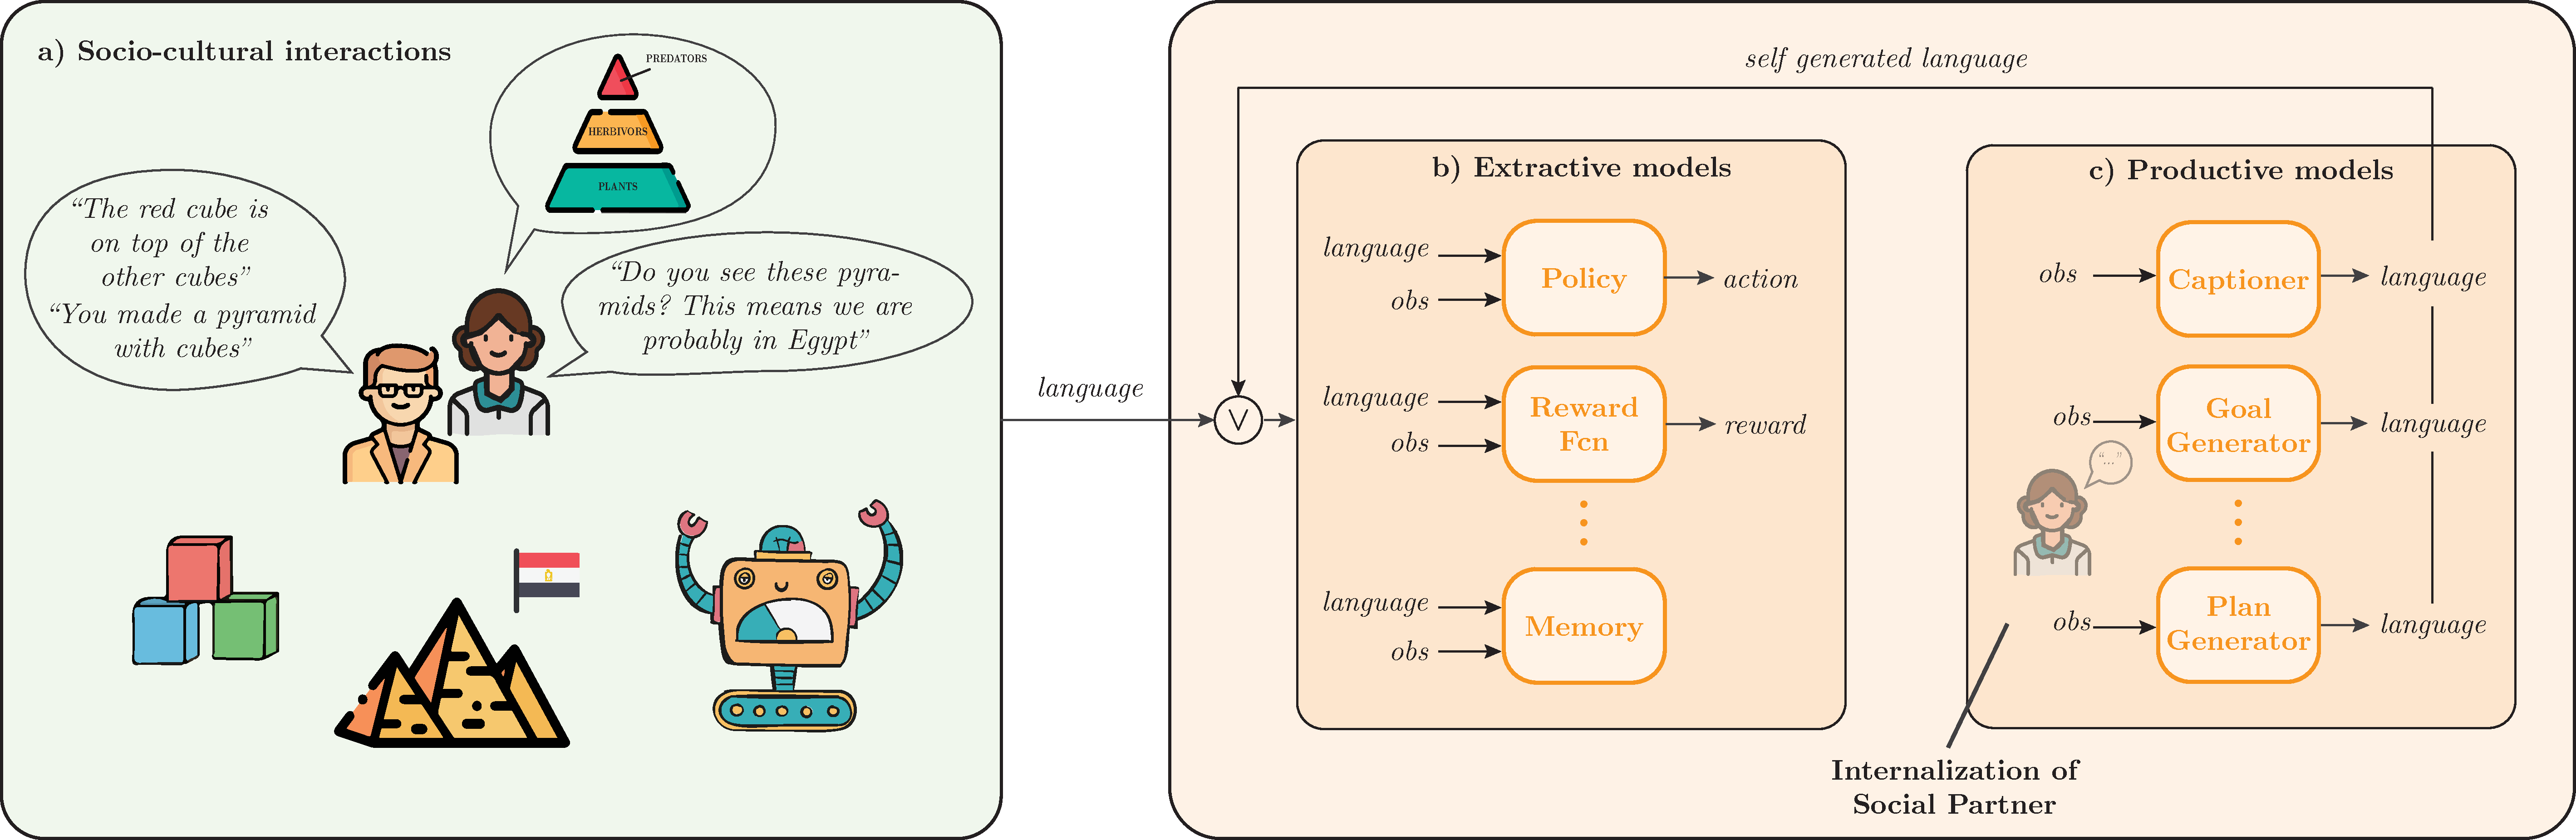
\includegraphics[width=1\linewidth]{perspective/extractive-productive-v3.pdf}
    \caption{\small The three components of Vygotskian autotelic agents: socio-cultural interactions, linguistic extraction and internalized linguistic production. Vygotskian autotelic agents are immersed into rich socio-cultural worlds where they experience a variety of linguistic feedback including descriptions, explanations, or metaphors (a). They can exploit information from linguistic structures and content by conditioning their internal modules on this feedback (b, extractive models). Finally, they learn to internalize social interactions by training productive models of language to generate feedback similar to the one they receive from others (c, productive models). This offers agents the autonomy to build their own cognitive tools, bootstrapped by socio-cultural language.}
    \label{fig:extractive_productive}
\end{figure}
\vspace{.4cm}


% % % % % % % % % % % % % % % % % % % % % % % % % % % % % % % % % % % % % % % % % % % % 
% Section: Extraction of Regularities from Language
% % % % % % % % % % % % % % % % % % % % % % % % % % % % % % % % % % % % % % % % % % % % 
\subsection{Exploiting Linguistic Structure and Content}
\label{sec:extraction}

In its vocabulary, syntax and narratives, language offers both powerful computational tools for thinking and important cultural knowledge about the world. According to Dennett's thesis, mere exposure to language can already help agents rewire their inner processes and develop new abilities. Recent advances in \ai seem to support that idea.

\textbf{Learning to abstract and generalize.} Exposition to linguistic labels is known to facilitate category learning in humans,\cite{waxman_words_1995, yoshida_sound_2003} but also in machines.\cite{lupyan_carving_2005} As Mirolli and Parisi defend, the repeated occurrence of a linguistic label (\textit{red} in their example) leads to the conflation of internal representations associated with that label (red things) which, in turn, facilitates further classifications based on the linguistic attributes.\cite{mirolli_towards_2011}

We see a similar effect in \rl agents targeting linguistic goals. The exposure to aligned instructions and trajectories seems to reshape the internal representations of the agent contained within its action policy. The policy is a neural network-based function conditioned on the agent's instruction that maps the current state of the world to its next actions. By \textit{internal representations}, we mean representations computed within the layers of the policy to facilitate the final decision-making. When repeatedly asked to grasp \textit{red objects}, the policy learns to focus on objects' colors to facilitate action selection.\cite{hill_emergent_2019,colas_language_2020} \textit{Red} is an abstraction over a continuous space of colors. It is first cultural, outside of the agent, but gets progressively internalized within the agent via a combination of linguistic exposure and decision-making. 

Exposed to a diversity of instructions, agents gain new cognitive abilities. The first is \textit{abstraction}. Linguistic autotelic agents can reach and make sense of abstract  relational goals ``\textit{sort objects by size},''\cite{jiang_language_2019} ``\textit{put the cylinder in the drawer},''\cite{lynch_grounding_2020} sequential goals ``\textit{open the yellow door after opening a red door},''\cite{chevalier-boisvert_baby-ai_2019} or even learning goals ``\textit{is the ghargh edible?}.''\cite{yuan_interactive_2019} Whereas handling abstract goals used to require engineers to hard-code specific goal representations and reward functions within the agent,\cite{curious,team2021open} linguistic goals offer abstraction via simple linguistic interactions.\cite{bahdanau_learning_2019,colas_language_2020} Once abstractions have been distilled within the representations of the agent, they can be leveraged to augment its exploratory capacities. Searching for novelty in a space of abstract linguistic descriptions of the world is indeed more efficient than searching for novelty in low-level sensorimotor spaces which could be trivially triggered by leaves moving in the wind or TV noise.\cite{tam2022semantic, Mu2022ImprovingIE}

A second cognitive ability is \textit{systematic generalization}. Language-instructed agents indeed seem to demonstrate the ability to generalize to new instructions obtained by systematic recombinations of instructions they were trained on.\cite{hill_emergent_2019} For instance, agents that learned to \textit{grasp blue objects} and \textit{put green objects on the table} can directly \textit{grasp green objects} and \textit{put blue objects on the table}.\cite{Hermann2017, chevalier-boisvert_baby-ai_2019, bahdanau_learning_2019, hill_emergent_2019, hill_human_2020, colas_language_2020, sharma2021skill, karch2021grounding} This ability can either be encoded in learning architecture through the use of modular networks (neuro-symbolic approaches), or emerge spontaneously in plain networks under the right environmental conditions.\cite{hill_emergent_2019} Although sometimes the world does not conform to strict linguistic compositionality, systematic generalization still supports good priors\,---\,\eg \textit{feeding the cat} is not a strict transposition of \textit{feeding the plant} but they still share similarities (bringing supplies to the cat/plant).\cite{colas_language_2020}

\textbf{Learning to represent possible futures.} After being exposed to aligned trajectories and linguistic descriptions, agents can generate concrete examples of abstract descriptions. The \decstr approach, for example, trains a generative world model to sample from the distribution of possible future states matching a given abstract linguistic description.\cite{akakzia_grounding_2021} This simple mapping supports \textit{behavioral diversity}, the ability to represent different possible futures so as to select one to pursue. Similar setups could leverage \dalle, an impressive text-to-image generative system.\cite{ramesh_zero-shot_2021,ramesh2022hierarchical} Trained on pairs of images and compositional descriptions, \dalle can generate high-quality images from the most twisted descriptions humans can think of. The exposition to compositional language, paired with sufficiently powerful learning architectures and algorithms leads to impressive visual composition abilities that could be put to use to generate visual goals or to represent possible futures in embodied and situated agents. 

\textbf{Learning to decompose tasks.} Vygotsky and others discovered that children's use of private speech helps them increase self-control and is instrumental to their capacity to reason and solve hard tasks.\cite{vygotsky_thought_1934, berk_why_1994} The ability to formulate sentences like ``at the left of the blue wall,'' for instance, predicts spatial orientation capacities in such contexts, while interfering with adult's inner speech via speaking tasks hinders theirs.\cite{hermer-vazquez_language_2001}

Language indeed contains cues about how to decompose tasks into sub-tasks, \ie how to \textit{generate good plans}. Although \textit{gharble} is a made-up word, \textit{fry the gharble} probably involves a preparation of the gharble (\eg peeling, cutting), some sort of oil and a frying pan.\cite{yuan_interactive_2019} \textit{Draw an octogon} contains cues about the decomposition of the task: \textit{octo} means 8, so we should probably do something 8 times, etc.\cite{wong_leveraging_2021} Recent \ai approaches leverage these regularities by training \textit{plan generators} from linguistic task descriptions.\cite{jiang_language_2019, chen_ask_2021, sharma2021skill, mirchandani2021ella, shridhar_alfworld_2021, wong_leveraging_2021} Among them, Wong et al.\, use plan generation as an auxiliary task to train a drawing policy.\cite{wong_leveraging_2021} Generating plans to solve a particular drawing task helps shape the internal representation of the main policy which, they find, favors abstraction and generalization in the main task. Interestingly, language only shapes representations and is not required at test time, in line with the requirement thesis of Dennett.

Inspired by video games of the 80s such as \textit{Zork}, text-based environments define purely linguistic goals, actions and states.\cite{cote_textworld_2018, das_embodied_2018, yuan_interactive_2019} Training a policy in such environments can be seen as training a plan generator in a linguistic world model, \ie training an inner speech to generate good task decompositions. This idea was exploited in \textit{AlfWorld}, where a pre-trained plan generator is deployed in a physical environment to generate sub-goals for a low-level policy.\cite{shridhar_alfworld_2021} Here, the abstraction capabilities of language help the plan generator solve long-horizon tasks.

The above approaches echo the thesis of Dennett (Section~\ref{sec:4views}): the mere exposure to structured language, once internalized within internal modules (reward function, policy, world model) strongly shapes inner representations in new ways and supports new cognitive functions (abstraction, future states generation, compositional generalization, task decomposition, etc).

 %Other methods take a complementary approach: they train advice-conditioned low-level policies and distill them into high-level task policies via supervised learning.\cite{watkins2021teachable}
\textbf{Learning from cultural artefacts.} Large language models (\llm) are trained on huge quantities of text scrapped from the internet: Wikipedia, forums, blogs, scientific articles, books, subtitles, etc.\cite{devlin2019bert,brown2020language} As such, they can be seen as \textit{cultural models} that contain information about our values, norms, customs, history, or interests.\cite{hershcovich_challenges_2022,arora2022probing} This represents a great opportunity for autotelic agents to learn about us, align with us, and better navigate our complex world. So far, only very little research has leveraged that opportunity. An example is the use of a trained \llm to act as a zero-shot planner, \ie a plan generator.\cite{huang2022language} Plugged with an interactive agent, the language model is used to generate sub-goals for the agent to solve the main task. Another work extracts information about complex time-extended behaviors from an \llm by asking it to score the actions available to the agent.\cite{ahn2022doasican}. Finally, the MineDojo framework\cite{fan2022minedojo} proposes to caption thousands of YouTube videos of humans playing Minecraft using GPT-3\cite{brown2020language}, generating creative high-level tasks as well as low-level linguistic guidance for embodied agents. Challenge~\#3 of Section~\ref{sec:challenges}  discusses more opportunities to harness these cultural models for open-ended skill discovery. 

% % % % % % % % % % % % % % % % % % % % % % % % % % % % % % % % % % % % % % % % % % % % 
% Section : Internalization of Language Production
% % % % % % % % % % % % % % % % % % % % % % % % % % % % % % % % % % % % % % % % % % % % 
\subsection{Internalization of Language Production}
\label{sec:production}

Agents that internalize extractive models learn to exploit the information contained within linguistic vocabularies, structures and narratives. However, most of them require external linguistic inputs at test time and, thus, cannot be considered autonomous. Vygotskian autotelic agents reach autonomy by internalizing \textit{productive models}; \ie by learning to generate their own linguistic inputs, their own \textit{inner speech} (see Figure~\ref{fig:extractive_productive}, c). 

Inner speech can be understood as a fully-formed language: descriptions, explanations or advice to be fed back to extractive models; to serve as a common currency between cognitive modules (fully-formed inner speech).\cite{zeng2022socratic} But it might also be understood as \textit{distributed representations} within productive models, \textit{upstream from fully-formed language} (distributed inner speech). In the latter interpretation, linguistic production acts as an auxiliary task whose true purpose is to shape the agent's cognitive representations. Symbolic behaviors might indeed not require explicit symbolic representations but may emerge from distributed architectures trained on structured tasks, \eg involving linguistic predictions.\cite{mcclelland2010letting,santoro2021symbolic} 
In the literature, we found four types of productive models making use of either fully-formed or distributed inner speech: trajectory captioners, plan generators, explanation generators and goal generators. 

\textbf{Trajectory captioners.} Trajectory captioners are trained on instructive or descriptive feedback to generate valid descriptions of scenes or trajectories.\cite{cideron_higher_2020, zhou_inverse_2020, colas_language_2020, nguyen2021interactive, yan2022intra} In line with Vygotsky's theory, these agents internalize models of descriptive social partners. They generate an \textit{inner speech} describing their ongoing behaviors just like a caretaker would. Used as an auxiliary task (distributed inner speech), the generation of descriptions helps the agent shape its representation so as to generalize better to new tasks.\cite{yan2022intra} With fully-formed inner speech, agents can generate new multi-modal data autonomously, and learn from past experience via \textit{hindsight learning},\cite{andrychowicz_hindsight_2017} \ie the reinterpretation of their trajectory as a valid behavior to achieve the trajectory's description.\cite{zhou_inverse_2020, colas_language_2020, nguyen2021interactive}

\textbf{Plan generators.} Plan generators are both extractive and productive. Following the formalism of hierarchical \rl (\hrl), plan generators are implemented by a \textit{high-level policy} generating linguistic sub-goals to a low-level policy (executioner).\cite{dayan_feudal_1993, sutton_between_1999} Linguistic sub-goals are a form of inner speech that facilitates decision-making at lower temporal resolution by providing abstract, human-interpretable actions, which themselves favor systematic generalization for the low-level policy (see Section~\ref{sec:extraction}).\cite{jiang_language_2019, chen_ask_2021, shridhar_alfworld_2021} Here, agents internalize linguistic production to autonomously generate further guidance for themselves in fully-formed language (task decompositions). 

\textbf{Explanation generators.} Vygotskian agents can generate \textit{explanations}. Using the generation of explanations as an auxiliary task (distributed inner speech) was indeed shown to support causal and relational learning in complex \textit{odd one out} tasks.\cite{lampinen_tell_2021} Note however that this approach is neither embodied, nor autotelic.

\textbf{Goal generators.} Some forms of creativity appear easier in linguistic spaces because swapping words, compositing new sentences, and generating metaphors are all easier in the language space than in sensorimotor spaces. The \imagine approach leverages this idea to support \textit{creative goal imagination}.\cite{colas_language_2020} While previous methods were limited to generating goals within the distribution of past experience (\eg with generative models of states\cite{nair2018visual}), \imagine invents out-of-distribution goals by combining descriptions of past goals. These manipulations occur in linguistic spaces directly and are thus \textit{linguistic thoughts}; fully-formed inner speech (Carruthers' view). The problem of goal imagination, difficult to solve in sensorimotor space, is projected onto the linguistic space, solved there, and projected back to sensorimotor space (Clark's view). This, in turn, powers additional cognitive abilities. First, it powers a creative exploration oriented towards objects and interactions with them. Second, it enhances systematic generalization by widening the set of goals the agent can train on.\cite{colas_language_2020}

By internalizing linguistic production, \imagine generates goals that are both \textit{novel} (new sentences) and \textit{appropriate} (they respect linguistic regularities, both structures, and contents).\cite{runco_standard_2012} Social descriptions focus on objects, object attributes, and interactions with these objects. Imagined goals obtained by recompositions of social ones share the same attentional and conceptual biases, \eg by reusing semantic categories of a particular culture. Thus, cultural biases are implicitly transmitted to the agent, which forms goal representations and biases goal selection following cultural constraints.\cite{colas_language_2020}

Note that productive models are very rare in the literature. In the future, Vygotskian autotelic agents must learn to internalize productive models for all types of multi-modal feedback they encounter: advice, explanations, attention guidance, motivation, instructions, descriptions, etc. It is only by learning to generate this guidance for themselves that they may gain full control of their own behavior. The question of whether to use fully-formed or distributed inner speech remains open, as both strategies seem to find different use-cases. Because cultural models are biased, future agents will need to edit, correct, augment and generate their own interpretations of culture based on their individual experiences. How to efficiently steer language models in these ways remains a question to explore in future research. 


% % % % % % % % % % % % % % % % % % % % % % % % % % % % % % % % % % % % % % % % % % % % 
% Section : Discussion
% % % % % % % % % % % % % % % % % % % % % % % % % % % % % % % % % % % % % % % % % % % % 
\subsection*{Conclusion}
% The Discussion should be succinct and must not contain subheadings.

This perspective builds on the autotelic \rl framework inspired by the Piagetian tradition to propose a complementary view motivated by Vygotsky's work: a \textit{Vygotskyan Autotelic AI}. Recent works at the intersection of deep \rl and \nlp present promising first steps, but a lot remains to be done. Vygotskian autotelic agents will interact with us and with our culture, exploit linguistic structures and content and finally internalize social interactions to serve as the basis of their future cognitive functions: abstraction, compositional thinking, generalization or imagination. 

Vygotskian Autotelic \ai opens a new research program with exciting opportunities. The current \nlp revolution can be harnessed to design more interactive and teachable agents. As they interact with humans and their peers in rich socio-cultural worlds, they will learn to leverage cultural and linguistic knowledge to bootstrap their cognitive development, and may eventually contribute back to our shared cultural evolution. This perspective uncovers an important challenge: how will we train and leverage cultural models to align with the values of human cultures so as to educate ethical and useful artificial agents?

Dennett used the software/hardware metaphor to describe the impact of language on human brains.\cite{dennett_consciousness_1993} Current \ai research mostly focuses on \textit{hardware} by asking \textit{how can we design better learning architectures and algorithms?} In complement, this paper suggests to focus on \textit{software} as well: \textit{How can we build the right socio-cultural bath which, combined with efficient hardware, will allow the emergence of a more human-like \ai}?



